% v2-acmsmall-sample.tex, dated March 6 2012
% This is a sample file for ACM small trim journals
%
% Compilation using 'acmsmall.cls' - version 1.3 (March 2012), Aptara Inc.
% (c) 2010 Association for Computing Machinery (ACM)
%
% Questions/Suggestions/Feedback should be addressed to => "acmtexsupport@aptaracorp.com".
% Users can also go through the FAQs available on the journal's submission webpage.
%
% Steps to compile: latex, bibtex, latex latex
%
% For tracking purposes => this is v1.3 - March 2012

\documentclass[prodmode,acmtochi]{acmsmall} % Aptara syntax

% Package to generate and customize Algorithm as per ACM style
\usepackage[ruled]{algorithm2e}
\renewcommand{\algorithmcfname}{ALGORITHM}
\SetAlFnt{\small}
\SetAlCapFnt{\small}
\SetAlCapNameFnt{\small}
\SetAlCapHSkip{0pt}
\IncMargin{-\parindent}

\usepackage{todonotes}

% Metadata Information
\acmVolume{0}
\acmNumber{0}
\acmArticle{0}
\acmYear{0}
\acmMonth{0}

% Copyright
%\setcopyright{acmcopyright}
%\setcopyright{acmlicensed}
%\setcopyright{rightsretained}
%\setcopyright{usgov}
%\setcopyright{usgovmixed}
%\setcopyright{cagov}
%\setcopyright{cagovmixed}

% DOI
\doi{0}

%ISSN
\issn{0}

% Document starts
\begin{document}

% Page heads
\markboth{N. Reeves et al.}{Virtual Citizen Science: A Theoretical and Empirical Overview}

% Title portion
\title{Virtual Citizen Science: A Theoretical and Empirical Overview}
\author{NEAL REEVES
\affil{University of Southampton}
SERGEJ ZERR
\affil{University of Southampton}
ELENA SIMPERL
\affil{University of Southampton}}
% NOTE! Affiliations placed here should be for the institution where the
%       BULK of the research was done. If the author has gone to a new
%       institution, before publication, the (above) affiliation should NOT be changed.
%       The authors 'current' address may be given in the "Author's addresses:" block (below).
%       So for example, Mr. Abdelzaher, the bulk of the research was done at UIUC, and he is
%       currently affiliated with NASA.

\begin{abstract}
Virtual Citizen Science (VCS) describes a web-based approach, recruiting, training and managing large numbers of volunteers in gathering and analysing data for scientific research. Although offline citizen science is well established, VCS is a nascent, rapidly evolving field covering an ever-growing number of tasks and processes, with ongoing focus in research concerning understanding and improving the design and implementation of VCS projects. In this paper, we present the findings of a meta-analysis of a transdisciplinary sample of literature, drawn from 5 databases. We first seek to define and describe the nature and limits of VCS as an approach, offering examples of tasks and scientific goals, as well as challenges associated with current projects. We then describe contemporary research covering 4 themes elicited using a grounded theory-based analysis of literature: design, engagement, sociality and evaluation. Our work seeks to contribute to the growing awareness of the opportunities posed by VCS, while highlighting areas for further study and consideration, to improve and refine this evolving field as a means to enable further scientific research.
\end{abstract}


%
% The code below should be generated by the tool at
% http://dl.acm.org/ccs.cfm
% Please copy and paste the code instead of the example below. 
%
 \begin{CCSXML}
<ccs2012>
<concept>
<concept_id>10003120.10003121.10003126</concept_id>
<concept_desc>Human-centered computing~HCI theory, concepts and models</concept_desc>
<concept_significance>300</concept_significance>
</concept>
</ccs2012>
\end{CCSXML}

\ccsdesc[300]{Human-centered computing~HCI theory, concepts and models}
%
% End generated code
%

% We no longer use \terms command
%\terms{Design, Algorithms, Performance}

\keywords{Virual Citizen Science, Meta-analysis, Literature Review}

\acmformat{Neal Reeves, Elena Simperl, Sergej Zerr, 2016. Virtual Citizen Science: A Theoretical and Empirical Overview.}
% At a minimum you need to supply the author names, year and a title.
% IMPORTANT:
% Full first names whenever they are known, surname last, followed by a period.
% In the case of two authors, 'and' is placed between them.
% In the case of three or more authors, the serial comma is used, that is, all author names
% except the last one but including the penultimate author's name are followed by a comma,
% and then 'and' is placed before the final author's name.
% If only first and middle initials are known, then each initial
% is followed by a period and they are separated by a space.
% The remaining information (journal title, volume, article number, date, etc.) is 'auto-generated'.

\begin{bottomstuff}
This work is supported by ...

Author's addresses: 
\end{bottomstuff}

\maketitle

\section{Introduction}

Citizen Science, the involvement of volunteers in scientific research, is not a new phenomenon. Until the 19th century, the majority of scientific research was conducted by non-professional scientists \cite{miller2012history}. These early, pioneering citizen scientists collected and analysed scientific data as a hobby, while pursuing other forms of employment \cite{silvertown2009new}. While research has become the domain of trained experts, opportunities for citizen engagement in science have persisted in the form of Citizen Science projects which allow volunteers to contribute to scientific enquiry \cite{catlin2012citizen}. The advent of the web and the uptake of scientific approaches such as open science and crowdsourcing have increasingly allowed volunteers to use online tools to train and engage in real research \cite{bonney2009citizen,kobori2016citizen}. 

New scientific approaches are increasingly necessary to cope with the modern scientific process. The Sloan Digital Sky Survey generates hundreds of thousands of images, far more than can be processed using the traditional methods, where small groups or individuals would manually classify each image \cite{lintott2008galaxy}. Yet, computational systems may lack the accuracy or efficiency required to deal with such data, leading to the recruitment of large numbers of volunteer citizen scientists through web-based portals, who can complete classifications far faster than small teams could achieve, in the \textit{Galaxy Zoo} project  \cite{lintott2008galaxy}. Modern technologies generate vast volumes of data. The Large Hadron Collider generates 60 terabytes of data per day, necessitating new approaches to data analysis \cite{bryant2008big}. This has led to the use of citizen science campaigns, including the Zooniverse project \textit{Higgs Hunters}, to analyse the quantities of data produced \cite{nellist2016involving}.

This Virtual Citizen Science (VCS) is a rapidly evolving space, employed across an increasing number of scientific disciplines. One of the most successful projects, \textit{Galaxy Zoo}, launched in 2007 and has since grown into the largest platform for VCS, \textit{Zooniverse} with over 40 projects across 5 domains \cite{tinati2015designing}. Projects within the space of online citizen science make use of a wide variety of tasks \cite{tinati2015designing} and goals \cite{wiggins2011conservation,wiggins2012goals}. 

Despite its potential, VCS is not without its challenges. While volunteers may be able to assist in generating data for scientific research, ensuring the validity of such data is a complex issue \cite{wiggins2011conservation}. Furthermore, generating such data necessitates attracting and motivating vast numbers of volunteers to participate within a project \cite{tinati2015designing}. Successful application of VCS approaches requires significant consideration of design principles across a range of areas, which are often at odds with the small and highly specialised science teams behind citizen science projects \cite{bonney2009citizen,tinati2015designing}. 

In this paper, we present a meta-analysis of literature related to virtual citizen science, drawn from a transdisciplinary set of sources. This meta-analysis surrounds five themes, elicited through a grounded theory-based approach: Project types, Design, Volunteer Engagement, Sociality and Communication, and Evaluation. For each theme, we outline a synthesis of research findings drawn from the literature, while making recommendations for the design and implementation of VCS projects. We conclude by identifying and outlining a number of opportunities for future research, elicited through a synthesis of our findings.

%This paper describes a meta-analysis of literature related to virtual citizen science, drawn from a transdisciplinary set of sources. We seek to clearly define VCS as a concept, describing VCS tasks, projects and scientific aims, while distinguishing related, but distinct areas with similar approaches. We present the results of a grounded theory approach, aimed to elicit key research themes and areas in the wider literature. We first present a definition of VCS, synthesised from the wider literature, alongside examples of scientific endeavours making use of VCS approaches. Secondly, we identify the challenges associated with VCS approaches. We then present findings surrounding 4 key themes identified during the review process: Design, Engagement, Sociability and Evaluation. 

\section{Background}

In this section, we present background concepts which describe the scope of our research. We first outline Virtual Citizen Science as an approach, describing the main forms it may take. We then highlight related, but distinct concepts, to clarify the areas which we analysed within our work. Furthermore, we identify previous work which has informed our research, while outlining how we built upon this work to conduct our own analysis. 

\subsection{Virtual Citizen Science}

Virtual citizen science is a diverse field, with multiple task types and approaches. In addition, VCS is itself a subtype of a broader spectrum of citizen science initiatives and volunteer engagement in scientific research. It is important to highlight and outline what we refer to when we talk of 'virtual citizen science'. We divide VCS into two broad classifications, in keeping with the approach specified by \cite{tinati2015designing}. Data collection refers to those tasks where volunteers contribute data and entities such as images to enable their use in scientific research. Data analysis, conversely, refer to those tasks where volunteers are given entities or other forms of data to analyse, producing further data or metadata to prepare these entities and associated metadata for further research.

\subsubsection{Data Collection}
Data collection tasks, similar to more traditional CS initiatives, require citizens to gather data or entities such as images, audio-recordings or videos, to enable scientific research. These projects cover tasks such as observation, measurement and sample collection described by Wiggins and Crowston's task typology \cite{wiggins2012goals}. Unlike in more traditional CS approaches, volunteers receive training through technology-mediated methods, such as tutorials, videos or technology-mediated communication with professional scientists or peers, either in addition to or in place of face-to-face training. Data collection may include the submission of photos, recordings, textual posts, gps data, the use of specifically designed apps or the completion of a survey, among other tasks. More simplistic projects correspond to the 'crowsourcing' level described by Haklay, where volunteers act as sensors, collecting data through, for example, smartphones \cite{catlin2012citizen,haklay2013citizen}.

Due to the nature of data collection tasks, the task is rooted in a real world location. Volunteers carry out offline tasks, using web-based technology to submit data \cite{wiggins2011conservation}, from processes such as surveying birds within one's own garden, or by recording physical location, to enable the tracking of organisms \cite{mason2012tiger} or natural phenomena\cite{liu2011going}.

The VCS project eBird is an example of a data collection project. Launched in 2002, eBird is one of the largest projects\cite{yu2010modeling}, with over 500,000 volunteers \cite{price2011carolina}. eBird leverages the hobby of amateur birdwatchers, encouraging volunteers to submit their observations to an online database and in doing so, aid scientific research \cite{yu2010modeling} \cite{wood2011ebird}. Volunteers within eBird contribute vast amounts of data, with 1.5 million contributions from within North America in 2010 \cite{yu2010modeling}, with 92,000 observations submitted each day \cite{o2014harnessing}. The project focus has grown from North America during initial stages of the project, now covering the globe \cite{catlin2012citizen}. Due to the visualisations available within the project, volunteers benefit from the increased accessibility of bird watching data \cite{catlin2012citizen} (see \ref{figure:eBird}). Observations submitted to eBird are used in a range of fields, including statistics, biology and computer science \cite{roy2012understanding}.

\begin{figure}[t]
\centering
\includegraphics[scale=0.2]{eBirdint}
\caption{Map visualising observations recorded within the eBird project}
\label{figure:eBird}
\end{figure}

\subsubsection{Data Analysis}

Data analysis tasks make up one distinct subset of VCS tasks. Such tasks make use of human computation to  produce metadata as a means of classifying or clarifying data or entities such as images for further analysis and research. Entities may take a variety of forms, such as images, videos, sound recording, graphs, text fields or even solveable puzzles. The tasks attached to these entities vary between fields of study, projects and platforms but include:

\begin{itemize}
  \item Cataloguing - Classifying items by characteristic
  \item Mapping - Mapping structures within images
  \item Transcribing - Digitizing text fields
\end{itemize}

%Morecitationshere add numberr of projects todo number of entities here
A key feature of data analysis VCS tasks is crowdsourcing. Tasks include vast numbers of entities. As a quality control measure, tasks require multiple classifications for each entity. As a result, such initiatives must appeal to large numbers of volunteers \cite{tinati2015designing}, over a million volunteers in the case of the largest data analysis VCS platform Zooniverse \cite{luczak2015resources}. 

Unlike data collection projects, which are rooted within physical locations, data analysis projects are location independent. Users do not need to make observations or measurements from physical objects, allowing volunteers to contribute at home. However, data analysis projects can be considered rooted in a virtual space, requiring users to contribute through a given website.

Galaxy Zoo is arguably one of the most well known data analysis VCS projects \cite{wiggins2011conservation}. First launched in 2007, initial early modest estimations for classifications were quickly surpassed, leading to the development of Galaxy Zoo 2. Now in its fourth incarnation, Galaxy Zoo has generated millions of classifications across 1.5 million entities from over 300,000 volunteers \cite{tinati2015designing}. The project aims to generate morphological classifications of galaxies photographed within the Sloan Digital Sky Survey \cite{galloway2015galaxy}. Users classifications represent only part of the research process, which makes use of more traditional, scientist-led methods to analyse data from the classified images \cite{madison2014commons}.

\begin{figure}[t]
    \centering
    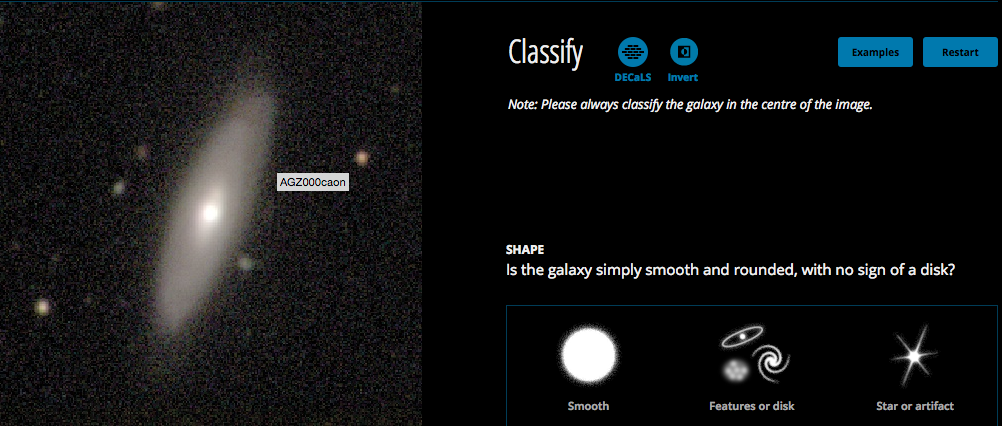
\includegraphics[scale=0.3]{Gzooface}
    \caption{Galaxy Zoo classification interface}
\end{figure}

\subsection{Related Concepts}

In addition to data collection and data analysis, a number of other task types have been associated with citizen science.

Open Science is a term discussed alongside citizen science \cite{morzy2014ict}. Similar to CS, open science seeks to engage members of the public in scientific research, ensuring data is available to the public. However, while the goals of both OS and CS may be similar, open science is not necessarily a form of citizen science, as data in open science projects may not be gathered or analysed by volunteers \cite{morzy2014ict}. There are, however, VCS projects which make use of open science approaches, such as OpenPhylo, an open science approach to multiple sequence alignment \cite{kwak2013open}.

Similar to mobile VCS are volunteered geographic information-based projects, which rely on users submitting geographical data for mapping and research purposes \cite{blatt2015benefits}. Data may be submmitted through GPS or manually entered by users. While there are similarities between VCS and VGI, in particular the elements of crowdsourcing and data collection, we believe that the key difference involves the use of contributed data. VCS data is explicitly used for scientific research, while VGI projects may be used for scientific research (in which case a project is both VGI and VCS) or for alternative purposes \cite{blatt2015benefits} (for example, compare \cite{foster2015volunteered} and \cite{poore2013metadata}). Despite this, VGI is sometimes described as synonymous with VCS (see, for example: \cite{sui2013volunteered} \cite{sui2012crowdsourcing}).

Volunteered computing describes a variety of project where users are largely passive. Volunteers run software on their computer or other device, which utilises the computing power of the device to carry out scientific analysis processes. Such projects are unique when compared with other forms of VCS, where technology is largely passive, filling an administrative role and volunteers carry out active tasks, collecting or gathering data. Whether such projects count as VCS is a point of some divergence in the surveyed literature (see \cite{haklay2013citizen,morzy2014ict,nov2014scientists} for example). We take the view that due to the passive nature of volunteers in such projects, volunteered computing cannot be considered a form of virtual citizen science. 

\section{Related Work}

While we note a lack of metastudies concerning virtual citizen science, a number of metastudies have explored citizen science at a broader level. In this section, we outline work related to our own research, which informed our analysis and which we drew from and built upon in order to complete our meta-analysis. 

Kullenberg and Kasperowski completed a meta-analysis of citizen science within the Web of Science repository, focussing on the scientific aims and disciplines \cite{kullenberg2016citizen}. The authors drew on two datasets, one of 1935 publications and one of 633 publications, in a bid to identify a specific definition of citizen science, comparing existing and conflicting definitions present within the literature. In addition, Kullenberg and Kaspeowski identify aims and objectives which may motivate the use of citizen science approaches such as engaging volunteers in the scientific process and political lobbying. In contrast, our research aims to explore virtual citizen science, a specific form of citizen science endeavour, drawing on a larger number of sources and considering further concepts such as design, sociality and empirical literature. Kullenberg and Kasperowski's work was valuable in understanding the citizen science space more broadly, characterising the types of research that we could expect to see. Furthermore, this outline of existing definitions and outlines of citizen science was an essential aid in allowing critical consideration of the literature identified within our survey methodology for relevance to citizen science.

We also note reviews of specific forms of citizen science research. Conrad and Hilchey completed a review of literature associated with environmental-monitoring initiatives within citizen science, identifying the types of initiative, administrative structures, benefits, challenges and potential recommendations associated with this distinct form of CS \cite{conrad2011review}. Our work considers similar concepts, but within a virtual citizen science context, rather than the physical, community-led context associated with environmental-monitoring. 

Similar to our work is the work of Catlin-Groves, who reviewed the 'citizen science landscape', identifying the differing types of project and initiatives in action within CS \cite{catlin2012citizen}. In addition, the author considers Web 2.0, Trust and Reliability and Shifting Paradigms within a CS context. In contrast to this, our work considers Virtual Citizen Science, a specific subset of CS, in more detail, situating it within the broader spectrum of Citizen Science approaches, while highlighting recommendations for design and for further research. 

Seaborn and Fels carried out a meta-analysis of gamification literature, drawing on 30 papers covering 31 systems \cite{seaborn2015gamification}. This analysis focused on both theoretical reviews of gamification and empirical analysis of gamification applications in live projects and practical observations of participants. The authors drew upon a cross-section of disciplines in order to carry out their analysis, identifying an evolving common conceptualisation of gamification, as well as points of departure in the literature. Similar is the work of Hamari et al, who carried out a literature review of empirical studies surrounding gamification in order to assess the success of gamification as an approach \cite{hamari2014does}. We use a similar approach in the area of virtual citizen science. These works was of particular use in designing our methodology, surrounding the literature search process.

%Third here - That paper about 'managing' and reviewing management of CS projects

%Catlin-Groves - citizen science landscape paper

\section{Methodology}

In order to conceptualise and create an overview of research surrounding VCS, we conducted a survey of contemporary literature. The aim of this survey was to identify current research surrounding the implementation and use of VCS as a research methodology, as well as research being conducted with VCS methods. To this end, the survey utilised a meta-synthesis approach, drawing on a range of qualitative and quantitative sources. In order to ensure a transdisciplinary overview of VCS and associated research, we drew on 5 different databases of literature: JSTOR, Scopus, Web of Science, PubMed and Google Scholar. This selection of databases was informed by the work of Seaborn and Fels, who carried out a multidisciplinary survey of literature associated with gamification, with similar goals to our research \cite{seaborn2015gamification}.

\subsection{Survey Process}

In order to carry out the literature survey, we selected 5 databases: Google Scholar, JSTOR, PubMed, Scopus and Web of Science. These databases were chosen in order to generate a transdisciplinary sample of VCS literature, an important objective given the variety of disciplines identified in the citizen science metastudy conducted by Kullenberg and Kasperowski \cite{kullenberg2016citizen}. Across databases, we used common search terms wherever possible, aiming to identify literature which used the terms virtual, online or digital citizen science. Where possible, we searched databases using abstracts, titles and keywords. In cases where this was not possible, we used the closes approximate (e.g., topic words - see figure 1). This led to a total of 1062 results. 
%In order to carry out the literature survey, we initially selected 4 repositories: JSTOR, PubMed, Scopus and Web of Science. These databases were chosen in order to generate a transdisciplinary sample of VCS literature, an important objective given the variety of disciplines identified in the citizen science metastudy conducted by Kullenberg and Kasperowski \cite{kullenberg2016citizen}. 
%Across databases, we used common search terms, aiming to identify literature which used the terms virtual, online or digital citizen science. Due to restrictions in the search tools provided, it was not always possible to apply the same restricting factors to these searches. Where possible, we searched databases using abstracts, titles and keywords. In cases where this was not possible, we used the closest approximation (e.g., topic words - see figure 1). This search process generated 538 results, but a number of issues were identified. The PubMed and JSTOR databases returned only 4 and 9 result respectively, the majority of which were unrelated to VCS. Furthermore, a large number of duplicate results were generated between the Scopus and Web of Science services - a total of 165 duplicates.

%Therefore, we turned to Google's Scholar service to supplement the survey. We selected Google's Scholar database due to its large size and the diverse range of topics and disciplines represented within the database. Due to the relative simplicity of the advanced search feature available in Google Scholar, search terms had to be modified. This database returned a further 515 results, of which 303 were determined to be unique.

\subsection{Selection Criteria}

Having identified a body of literature, we applied a number of exclusion criteria to generate a suitable sample for study. Firstly, all duplicate results were removed from the list of literature. Subsequently, each of the remaining results was assessed for relevance, based on its applicability to virtual citizen science. Those literature items which dealt with solely offline forms of citizen science, forms where online components could not be identified, or other concepts entirely were removed from the list. Furthermore, we excluded any publications which simply used VCS data, rather than discussing VCS theory, systems or concepts. We identified a large number of publications dealing with a relatively small number of projects. Where multiple publications referred to the same project, we prioritised literature which provided the most in-depth 

At this point, having identified a smaller sample, a grounded theory approach was employed to identify relevant themes and subject areas within the sample, while eliminating outliers and potentially irrelevant topics. Initially, literature was coded at the level of title and abstract, to identify general themes. Following this, publications were then analysed in depth, with items assigned to themes. Papers which did not align to themes and which were unsuitable for this analysis were then removed. While the process of removing papers included some element of subjectivity, objective criteria were employed: papers which, when coded, were identified as having unique categories, categories unrelated to defining or analysing VCS, or made only passing mention of VCS were considered to be outliers or irrelevant and were therefore chosen for removal at this stage.

\begin{table}
    \tbl{Databases and search terms used and results generated.}{
    \begin{tabular}{p{3cm}|p{7.5cm}lap{2cm}}\hline
    \textbf{Repository} & \textbf{Search terms} & \textbf{Results}\\ \hline
    JSTOR & ((ab:("online" + "citizen science") OR ab:("digital" + "citizen science") OR ab:("virtual" + "citizen science")) & 9\\ \hline
    Scopus & TITLE-ABS-KEY (``online'' + ``citizen science'') OR TITLE-ABS-KEY (``digital'' + ``citizen science'') OR TITLE-ABS-KEY (``virtual'' + ``citizen science'') & 290\\ \hline
    Web of Science & TOPIC:(``online'' + ``citizen science'') OR TOPIC:(``digital'' + ``citizen science'') OR Topic:(``virtual'' + ``citizen science'') & 253\\ \hline
    PubMed & (("digital citizen science"[Title/Abstract]) OR "virtual citizen science"[Title/Abstract]) OR "online citizen science"[Title/Abstract] & 4\\ \hline \hline
    Google Scholar & ``online citizen science'' OR ``virtual citizen science'' OR ``digital citizen science'' & 496\\ \hline
    \end{tabular}}
\label{table:searchterms}
\end{table}


\subsection{Limitations}

We noted the use of both "online citizen science" and "virtual citizen science" within previously studied literature, as well as a less common but still significant use of "digital citizen science". Similarly, a number of publications made use of the more general term "citizen science", without distinguishing the more recently evolving web-mediated form of citizen science from the more traditional, offline variety. Still other publications appeared to make a distinction between digital citizen science as a technology-mediated, but generally offline method and online citizen science as a specifically web-mediated method, with virtual citizen science being used interchangeably. 
A further limitation lies in the rate of CS data publication. Data generated in CS initiatives take a long time to reach publication, if indeed they are published at all \cite{theobald2015global}. As a result, identifying newer VCS projects in order to describe and define the space was a key difficulty. This is particularly the case with platforms such as the Zooniverse, which launches new projects each year with an increasing variety of disciplines, contexts and tasks \cite{tinati2015designing}.

%334 projects = 32%
Despite the 1062 publications identified during original sampling, a large proportion (~32\%) of publications were duplicated between one or more databases. In addition, after removing duplicated publications, a further ~66\% of publications were deemed to be of little relevance to this analysis. One key reason for this was the large proportion of publications reporting results from a CS initiative, generally describing traditional, predominantly offline CS approaches. Similarly, a number of publications discussed design science related concepts, using VCS projects as examples, rather than focusing on VCS design.

In spite of our efforts to generate a multidisciplinary sample of publications, we note the dominance of three key application areas (Biological Sciences, Astrophysics and Climatology) and the dominance of HCI/Design Science with regard to project design. We believe this is due to the slow rate of publication, as mentioned, and due to the nature of VCS as a nascent, evolving field, necessitating research surrounding design and application at this stage. 

Despite these limitations, our work offers valuable insight into virtual citizen science as distinct from other, offline forms of citizen engagement in science. We believe our study represents the largest meta-analysis of literature in the area of citizen science. Furthermore, our work is the only meta-analysis to date with a focus on literature surrounding virtual citizen science, distinguishing research surrounding online, crowdsourced forms of citizen data collection and analysis from more traditional, offline forms of participation. 

\section{Virtual Citizen Science Theory}

Virtual Citizen Science refers to a diverse approach to scientific research, consisting of a wide variety of task types and scientific goals. Describing this approach concisely is a difficult task. Unlike traditional models of citizen science, VCS is a relatively nascent area, being intrinsically linked with the growth of the Web. Furthermore, the increasing availability of portable devices has let to emerging opportunities and provoked novel approaches to gathering data in VCS \cite{catlin2012citizen}. It is perhaps unsurprising, then, that VCS as a field is growing and evolving rapidly. Zooniverse, described as the largest single platform of VCS projects, has grown from a single project in 2007, reaching 37 projects across 7 domains in the space of just 7 years and continuing to grow rapidly \cite{luczak2015resources,tinati2015designing}. Within the literature, VCS is described alongside similar but distinct approaches such as open science, volunteered geographic information and volunteered computing further. 

This section outlines theory surrounding Virtual Citizen Science, in particular outlining the types of project, objectives and approaches associated with VCS, while also situating VCS in the larger spectrum of CS projects. For this purpose, we present findings surrounding the scope of VCS and its diversity. We highlight associated vocabulary, the methodological approaches used within projects and distinguish VCS from similar approaches which nonetheless hold key differences. We further explore examples of the scientific research conducted using VCS methods. 

%Despite a relatively large body of research surrounding applying and designing VCS to various contexts, defining VCS is somewhat challenging. Unlike traditional citizen science models, VCS is relatively nascent, relying as it does on the infrastructure of the Web as a means to attract participants. Despite this, it is also a fast moving, readily evolving field - Zooniverse, the largest platform of VCS projects, has grown from a single project in 2007, reaching 37 projects across 7 domains in the space of just 7 years and continuing to grow rapidly since \cite{tinati2015designing}\cite{luczak2015resources}. At the same time, the increasing availability of technologies such as smartphones and other portable devices has led to emerging opportunities and provoked novel approaches to VCS as a scientific methodology \cite{catlin2012citizen}. We note the coexistence of numerous similar terms (\textit{digital}, \textit{online} and \textit{virtual} citizen science) and a variety of associated tasks. Similarly, the presence of similar but distinct related terms used alongside VCS provokes further consideration about the boundaries between VCS and other online crowdsourcing initiatives. 
%Our first goal with this paper is to synthesise a definitions of VCS, drawing on points of similarity and any key points of divergence within the literature. Here we present findings from within the surveyed literature concerning the scope of the term VCS - the terminology used to describe VCS; the activities to which VCS has been applied; the areas described with the term VCS and to distinguish any similar but distinct terms identified within the literature. We conclude this section by drawing on these findings to produce a clear synthesis of VCS which reflects contemporary literature, while avoiding the ambiguity associated with the various terms and approaches used.  

\subsection{Terminology}
%todo citations

The surveyed literature does not agree on a common vocabulary for describing concepts in VCS. We note, for example, that there is no common term for this particular form of citizen science participation, with \textit{online}, \textit{virtual} and \textit{digital} citizen science all being used interchangeably within the literature, as well as simply citizen science. Furthermore, individual terms are used to cover multiple concepts - the word task may refer to particular interface features pertaining to participant actions (e.g., task interface), or to the individual actions carried out by the participants (e.g., the transcription task). For want of a common vocabulary and for purposes of clarity, we have defined a specific set of terminology for use in this paper, which can be seen in table \ref{table:terminology}.

\begin{table}[t]
    \tbl{Terminology for use}{
    \begin{tabular}{p{3cm}|p{7.5cm}|p{2cm}}\hline
    \textbf{Term} & \textbf{Definition} & \textbf{Example}\\ \hline
    \textit{Entity} & Data object contributed by and/or analysed by participants & Image, Video\\
    \hline
    \textit{Task} & Process carried out by volunteers when collecting and/or analysing data & Transcription\\
    \hline
    \textit{Project} & VCS system (includes microtask, community and associated features) & Galaxy Zoo\\
    \hline
    \textit{Platform} & Collection of projects with common domain & Zooniverse, CosmoQuest\\
    \hline
    \textit{Participant} & Individual Volunteer & N/A\\
    \hline
    \textit{Sociality Platform} & Space for interaction between volunteers and project scientists & Blog, Forum\\
    \hline
    \end{tabular}}
\label{table:terminology}
\end{table}

%Defining virtual citizen science is a difficult task. Within the papers surveyed, a wide variety of terminology is used, often interchangeably or with only subtle differences. The three most widely used terms are \textit{Online}, \textit{Virtual} and {Digital} citizen science - perhaps unsurprising, given the search terms used. While the three terms are not synonyms, all three terms are used to describe the VCS project Galaxy Zoo. \textit{Technology-mediated} science is a similar, but less popularly used term. In spite of the apparent distinction between traditional citizen science intiatives and more recent technologically-mediated VCS, the term citizen science is used to refer to traditional and modern contexts, further complicating the task of identifying VCS.

%In addition to differences between terms, there is a notable difference even within the use of a given term. The majority of the papers surveyed make use of 'virtual' citizen science to refer to virtual citizen science as a broad approach utilising technology as a method of delivering and mediating scientific tasks to large numbers of volunteers. However, Wiggins and Crowston \cite{wiggins2011conservation} describe a typology of online, crowdsourced CS projects that uses the term \textit{virtual} to describe a specific class of project, distinct in its independence from real world locations and the absence of offline collaboration. Conversely, a number of typologies and case studies describe tasks requiring collection of data from physical locations (see for example \cite{tinati2015designing}\cite{mason2012tiger}\cite{mattos2014mission}).

\subsection{Typologies}

Within the surveyed literature, we identified a variety of typologies, proposed to describe the VCS space, dividing projects based on scientific aims and task types at varying levels. Our findings suggest that there is no dominant framework, nor a commonly accepted set of factors from which to divide projects. In this section, we outline the typologies identified within our meta-analysis, before synthesising our own framework, as a foundation for outlining more varieties of VCS. 

Task type is a common distinguishing factor in VCS typologies. Tinati et al distinguish projects based on high level classifications of the tasks expected of users: data collection, data analysis and problem solving \cite{tinati2015designing}. While this framework describes problem solving as a separate process, our analysis suggests that it can also be a significant factor in motivating data collection and analysis through VCS, where more traditional methods were no longer adequate (see for example, \cite{curtis2014online,lintott2008galaxy}.

Data collection tasks in turn have been described more specifically by Wiggins and Crowston. Drawing on previous literature, they specify 3 project types based on the stages of scientific enquiry in which volunteers participate \cite{wiggins2012goals}:
    \begin{itemize}
        \item \textbf{Contributory} - Volunteers engage in data collection and occasionally data analysis or dissemination of results.
        \item \textbf{Collaborative} - Volunteers engage in data collection and the analysis of samples and data, occasionally also engaging in study design, interpretation and conclusion drawing or the dissemination of results.
        \item \textbf{Co-created} - Volunteers engage in all stages of the scientific process.
    \end{itemize}

Haklay similarly distinguishes engagement based on the extent to which volunteers are involved in the scientific process, dividing the space into four levels \cite{haklay2013citizen}. Level one describes 'crowdsourcing', where volunteers are mere sources of data, acting as sensors or volunteering computing power. Level two describes 'distributed intelligence', where volunteers carry out simple interpreting and analysis tasks. Moving beyond this is 'participatory science', a level at which volunteers are involved in defining the problem of study and carry out more complex data collection tasks than described in level one. The highest level is 'extreme citizen science', where volunteers are engaged at all stages of the process, similar to the co-created classification described by Wiggins and Crowston.

More specific is Wiggins and Crowston's further framework of ten task types based solely on the process which volunteers undertake to produce data or metadata \cite{wiggins2012goals}, consisting of actions which can be mapped to Tinati et al's more high level typology. These processes are: observation, species identification, classification/tagging, data entry, entity finding, measurement, sample collection, sample analysis, site selection, geolocation, photography and data analysis. Data analysis here refers to a more specific process than the general description given by Tinati et al, which covers processes such as classification and geolocation. 

A similar basis is used by Wiggins and Crowston, who divide projects based on aim, task and the nature of project administrators and audience:
    \begin{itemize}
        \item \textbf{Action} - Citizen-led interventions based on local environmental issues.
        \item \textbf{Conservation} - Scientist-led projects aiming to educate and encourage awareness and stewardship of natural resources.
        \item \textbf{Education} - Scientist-led projects where all project activities are entirely conducted virtually, independent of the physical environment.
        \item \textbf{Investigation} - Scientist-led projects requiring data collection from physical environment, at local, national or international level.
        \item \textbf{Virtual} - Scientist-led projects where education and outreach are the primary, rather than secondary, goals.
    \end{itemize}

A recurring characteristic noted in these typologies is a division between processes involving data collection from physical locations and processes involving data analysis, conducted solely in online environments. We therefore propose a simple typology of data collection vs data analysis, as a medium for defining VCS approaches and tasks. We believe this simplified system allows for the classifiction of projects based on task and location, allowing for a less fragmented definition than would result from more complex and subtle frameworks. 

\subsubsection{Games With a Purpose}

Games With A Purpose are a distinct subset of citizen science projects, described separately within the literature (see, for example: \cite{prestopnik2013data,prestopnik2014exploring}. These projects ask volunteers to analyse data through the medium of games and puzzles \cite{curtis2014online}. While all data analysis tasks may make use of gamified aspects, such as leaderboards, points and badges (see Gamification), GWAP differ in that the task presented to a user is explicitly a game or puzzle. 

Launched in 2008, FoldIt is an example of a GWAP, where volunteers complete puzzles to identify the process for folding proteins, a task difficult to conduct with more traditional computation methods \cite{curtis2014online} (see figure 4). Players' solutions to protein folding puzzles are rated, based on the energy required to produce proteins and the similarity to natural protein configurations, with points awarded accordingly \cite{curtis2015motivation}. The FoldIt game is online and multiplayer \cite{khatib2011algorithm}. Players may participate individually or in teams and may compete with others based on points scored \cite{curtis2014online} \cite{curtis2015motivation}. Players are encouraged to collaborate and discuss solutions with other volunteers through a live chat function, with the opportunity to use asynchronous communication platforms \cite{curtis2015motivation}. Due to the complex nature of the protein folding process, FoldIt is a relatively complex game when compared with other online multiplayer games and players are required to complete a lengthy process of 32 tutorial puzzles before reaching assessed puzzles \cite{curtis2015motivation}. Despite this difficulty, players have contributed to the development of protein folding algorithms surpassing previously published algorithms \cite{khatib2011algorithm}.

\begin{figure}[t]
\centering
\includegraphics[scale=0.3]{Foldint}
\caption{FoldIt puzzle interface \protect\cite{curtis2014online}}
\end{figure}



%Conversely, other typologies classify VCS projects by the task requested of users \cite{catlin2012citizen}. Tinati et al \cite{tinati2015designing} describe three types of VCS task: data collection, data analysis and problem solving. Wiggins and Crowston \cite{wiggins2012goals} further identify three types of data collection: contributory, collaborative and co-created. Projects are distinguished by the extent to which the public are involved in processes, from contributory tasks where volunteers are largely data collectors, to co-created tasks where users contribute throughout the scientific publication process. 
%\subsubsection{Social Media VCS}

%One relatively unique approach to data collection tasks is the use of social media to share and/or gather data for scientific research. The use of social media and social networking platforms such as Twitter has grown significantly in recent years \cite{newman2012future}. By identifying posts, comments or tweets related to a given subject, social media posts can be used to track or otherwise record the occurence of natural phenomena such as storm-related flooding \cite{liu2011going} or earthquakes \cite{wiggins2011conservation}. Social Media VCS differs from other data collection methods in that while users are actively contributing scientific data, such contributions need not stem from deliberate effort. In the area of flood mapping, for example, Twitter users already share information about flooding, although this unintentional data sharing may lack necessary information such as terminology and location or  may use vague descriptions \cite{liu2011going}.

%\subsubsection{Data Collection Case Study - eBird}

%\subsubsection{Data Analysis Case Study - Galaxy Zoo}
%todo all of these correct numbers here


%Users are presented with images of galaxies and a selection of simple questions designed to classify the galaxy within the image. Questions are asked one at a time, with the image for reference (see figure 2) Although the task contains eleven questions in total, the branching nature of the classification process limits the number of questions users are asked about each image (see figure 2).


%\begin{figure}[t]
%\centering
%\includegraphics[width=\columnwidth]{Gzootree}
%\caption{Diagram of branching question and answer structure in Galaxy Zoo \protect\cite{casteels2013galaxy}}
%\end{figure}

%Galaxy Zoo is arguably one of the most well known data analysis VCS projects \cite{wiggins2011conservation}. First launched in 2007, initial early modest estimations for classifications were quickly surpassed, leading to the development of Galaxy Zoo 2. Now in its fourth incarnation, Galaxy Zoo has generated \todo{x number} of classifications across \todo{x number} of entities from over \todo{x number} of volunteers. The project aims to generate morphological classifications of galaxies photographed within the Sloan Digital Sky Survey \cite{galloway2015galaxy}. Users classifications represent only part of the research process, which makes use of more traditional, scientist-led methods to analyse data from the classified images \cite{madison2014commons}. By 

%Introduce Wiggins and Crowston definition
%Explain how they view Virtual CS
%Explain how they distinguish Virtual from other 4
%Note that this distinction does not appear to hold up against other sources
%Describe rapid evolution of VCS (Tinati et al 2015 and ZV)
%In their Typology of Citizen Science, Wiggins and Crowston (2011) examined factors influencing design and citizen participation. Using a landscape sampling method, the authors Wiggins and Crowston then coded projects according to 80 facets. This research aimed to identify common characteristics across citizen science projects. After coding facets, projects were clustered in order to group and identify projects with similar characteristics.

%This process led to a total of 5 project types: Action; Conservation; Investigation; Education and Virtual.  Action projects generally concern localised research action, which is led by citizens rather than scientists. Conservation projects, tend to be regional rather than local and involve collaboration with larger organisations. Investigation projects concern those in which volunteers gather data from a physical environment and it is this type, which best fits the most traditional definition of citizen science. Education projects have education and outreach as primary project goals, rather than secondary goals which may occur in other projects and are similarly rooted within a location.

%Virtual projects are relatively unique within this typology, as such projects refer to those, which are computer-mediated, with no physical element attached – such projects are not localised. Ensuring the accuracy of results is a key challenge for virtual CS projects. In order to overcome this challenge, projects make use of repetition, with multiple users asked to complete the same classification. A further difficulty lies in designing tasks to ensure that they are motivating for users while also ensuring accurate and valuable contributions for scientific research. Wiggins and Crowston note that the variety of tasks for which a virtual CS-based approach can be used is relatively low and generally requires the design of relatively complex platforms in order to support the approach. It is noted that this approach requires the support of computer scientists is often required for the development of such platforms, an observation supported by Tinati et al (2014). 

%Catlin-Groves (2012) notes that despite these differences between more traditional CS approaches and the more modern, web-based approach, there are certain key similarities. Both traditional and modern approaches make use of a formal submission process, with submissions generally made inaccessible to users, generally until the point at which results are published. Catlin-Groves notes that even where data is open to volunteers, it is generally inaccessible in the sense that users cannot visualise or understand the significance of data, which has a negative impact on participation. This challenge can be transformed into a potential strength for virtual, web-based projects, through the use of visualisation portals and techniques. Such an approach was adopted by e-Bird in 2006, leading to a significant increase in the volume of user-participation.

%In addition to projects where users actively participate, Nov et al (2011) identify a futher type of computer-based CS project. These “Volunteer computer projects” ask volunteers to run specific software on their computers in order to solve specific problems through distributed computing. In such cases, volunteers play a largely passive role, at least within the research process. Rather than in the case of virtual projects identified by Wiggins and Crowston, where software platforms guide the contribution process, here the software takes full control of the research process and volunteers serve a largely administrative role. 
\subsection{Scientific Aims}

This section aims to describe some of the underlying scientific research aims held by particular virtual citizen science projects, to clarify the definition set out above. Our analysis identified a diverse range of projects, from varying disciplines and a full list of these goals is beyond the scope of this work. Instead, we seek to identify some of the common, recurring goals identified within VCS literature, providing an overview of the kinds of research conducted using VCS, to further clarify the space which our meta-analysis considers.

%Having defined VCS, our second aim is to describe the research aims associated with the use of VCS methodologies. To that end, we identified VCS projects and tasks within the surveyed literature. Three broad research topics accounted for the largest share of projects. These areas are: Biological Sciences, Astrophysics and Climatology and Disaster Tracking. 

\subsection{Data Collection}

\subsubsection{Species Tracking} % was subsubsubsection

A common scientific aim among data collection projects identified within the survey process concerns tracking organisms. These projects have a number of goals: volunteers may track species for conservation \cite{mattos2014mission,wiggins2011conservation}, identify the presence of invasive species for action by scientists \cite{mattos2014mission}, or assist scientists in tracking the presence and migration of species of interest \cite{swanson2015snapshot}, while also educating participants \cite{cunningham2012maryland}. Species tracking projects correspond largely to the conservation category specified by Wiggins and Crowston \cite{wiggins2011conservation}.

Species tracking projects cover a variety of scientific fields: botany \cite{mattos2014mission}, ornithology \cite{cooper2012natural,wiggins2011conservation}, herpetology \cite{o2014harnessing}, entomology \cite{mattos2014mission} and ecology \cite{mason2012tiger} were all identified within the sampled literature. The specific focus of such projects varies, from monitoring all reptile species across the state of Carolina \cite{price2011carolina}, to recording specific types of butterfly present in a localised region \cite{mattos2014mission}.

\subsubsection{Disease Tracking}

Similar to species tracking initiatives, disease tracking projects ask volunteers to record incidents of a particular illness. Aggregation of these incidents allows scientists to track and monitor the spread of illnesses, lending insight into disease characteristics, while allowing for action to be taken where necessary \cite{mattos2014mission}.

\subsubsection{Disaster Tracking}

VCS has been used to monitor, record and observe occurrences of natural disasters such as floods and earthquakes \cite{liu2011going,wiggins2011conservation}. These projects record individual events and the physical and social impact associated with such disasters. Similar to disease tracking, disaster tracking projects may also have a more humanitarian focus, allowing careful consideration of relief efforts in affected areas \cite{dittusanalysing}.

%Although the majority of mobile VCS projects identified are species tracking apps, a survey of nature-related apps on the Google Play Store conducted by Jepson and Ladle identified just 25 apps which allowed volunteers to upload observations to databases, with 33 total citizen science apps, suggesting such apps are rare \cite{jepson2015nature}.


%Other projects focus on herpetology, tracking reptile populations within localised geographic ranges \cite{cunningham2012maryland}\cite{o2014harnessing}. A wide variety of projects exist, from those focused on one form of reptile such as Frogwatch to broader geographical projects \cite{o2014harnessing}. Such projects serve the dual purposes of enabling effective conservation management of threatened species and education for project participants.

\subsection{Data Analysis}

\subsubsection{Digitisation}

Transcribing entities is an important step in enabling further scientific research. The \textit{Ancient Lives} project recruits volunteers to transcribe, measure and catalogue over 500,000 ancient Greek papyri, to enable their usage in humanities-based research \cite{williams2014computational}. In the field of history, \textit{Operation War Diaries} asks volunteers to transcribe diaries and reports kept by soldiers during World War One, digitising this data and allowing it to be shared more easily, enabling research \cite{towheed2015readers}. \textit{Notes from Nature} similarly leverages volunteer interest in transcribing data from museum collection labels, as a means to making such data freely available for scientific research purposes \cite{hill2012notes}. 

\subsubsection{Mapping}

Mapping physical structures present in entities is a common task in the astrophysics projects described within the literature. The \textit{CosmoQuest} platform recruits volunteers to map structures such as craters and boulders on images of the moon, asteroids and the planets Mercury and Mars \cite{gay2012cosmoquest}. Zooniverse's \textit{Moon Zoo} similarly maps craters and boulders \cite{joy2011moon}. Participants within the \textit{Milky Way Project} trace 'bubbles', structures related to nebula and star formation, seen in images of our own galaxy, allowing scientists to publish catalogues of these bubbles \cite{simpson2012milky}. While mapping generally involves geographical images, the \textit{Planet Hunters} project identifies planetary candidates orbiting stars by recruiting volunteers to trace 'transits', areas of low light activity corresponding to structures passing in front of a star, on to light curve graphs \cite{schwamb2014planet}.

%\subsubsection{Cataloguing}

\subsubsection{Puzzle Solving}

Common in Games With A Purpose, a subset of projects leverage the puzzle solving capabilities of participants to find solutions to problems which would be computationally expensive or inaccurate for current computing algorithms to solve \cite{lee2014rna}. EyeWire recruits participants in tracing neuron structures present in 3D images, to further neuroscience research \cite{curtis2014online}. FoldIt presents volunteers with puzzles representing protein folding patterns, enabling understanding of the factors involved in biological processes through digital models and the creation of more accurate algorithms \cite{khatib2011algorithm}. Similar algorithm development has been carried out in the GWAP EteRNA, which used solutions to RNA folding sequences contributed by volunteers to produce new algorithms with far greater accuracy than those previously available \cite{lee2014rna}.

\subsection{Summary}

Virtual Citizen Science is fundamentally defined by the process used to gather data or metadata and the purpose for which this data is used. Volunteers utilise the Web infrastructure to contribute data which they have gathered, or to engage with games, puzzles or other tasks as a means of generating metadata. VCS does not by necessarily require that volunteers be aware of their participation in research - data and observations shared by social media may be useful sources for scientific study. However, volunteers must \textit{actively} participate in the data or metadata production process, unlike volunteered computing, where volunteers are largely passive. While such approaches may also apply to other crowdsourcing-based areas such as VGI, it is the subsequent use of these data and metadata for scientific research that identifies this form of crowdsourcing as Virtual Citizen \textit{Science} and distinguishes it from other, volunteer-based crowdproduction initiatives. 

VCS has been employed in a wide variety of scientific research tasks, gathering and analysing entities and data for a broad variety of purposes. We divide these tasks into two high-level categories. 

Data collection recruit volunteers to gather data for scientific purposes, engaging volunteers in tasks such as tracking invasive, endangered or threatened species, tracking diseases or the impact of natural disasters. This enables scientists to use such data to manage conservation efforts, monitor the impact of particular phenomena and respond to situations in need of action. 

Data analysis projects recruit volunteers to assess entities and data, preparing them for use by scientists. Volunteers may transcribe text for digitisation, catalogue images for publication and further analysis, map structures to images or solve problems unsolvable with current computational models.

Unlike other forms of citizen science participation, where research is grounded in real world environments, virtual citizen science is carried out predominantly in online environments, using online tools and platforms to upload, analyse, share and visualise data. The level at which volunteers engage with the scientific process varies between projects, from simple contributory models, to co-created approaches where volunteers play a key role in planning, carrying out, producing and disseminating research.

VCS has been employed to enable a number of forms of research, from biological species tracking to digitisation of museum materials. A subset of VCS projects ask volunteers to complete puzzles representing biological models, to enable further understanding of their real-world counterparts. This wide spectrum of approaches and projects is likely to grow as new projects are proposed and existing  approaches are applied to new contexts and disciplines. 
%\subsection{Biological Sciences}

%The majority of initiatives identified are broadly identifiable as belonging to the Biological Sciences. This is in keeping with the findings of Kullenberg and Kasperowski, who identified biology, ecology and conservation as well as geographic information submission as key focal points of broader citizen science research \cite{kullenberg2016citizen}. Within the sampled literature, VCS projects made use of a combination of these approaches, often using geographic data to track and identify species for the purposes of conservation or ecology-related research. 

%\subsubsection{Ecology/Species Tracking}


%Ornithological projects make up the largest share of species tracking initiatives identified. The Cornell Lab of Ornithology hosts a variety of ornithology related projects, such as the (now complete) online survey My Yard Counts \cite{cooper2012natural}, educational focused project BirdSleuth \cite{wiggins2011conservation} or eBird as mentioned previously. Neighbourhood NestWatch focuses on identifying and observing nests in urban, suburban and rural contexts \cite{catlin2012citizen}. PredatorWatch is a similar survey hosted by the American Bird Conservancy \cite{cooper2012natural}.  

%

%Furthermore, botany is also a popular focus for species tracking apps. Invasive species tracking is a popular topic among botany projects, allowing volunteers to identify and track such species in order to enable professional scientists to take action \cite{mattos2014mission}.



%\section{Projects and Platforms}

%Virtual citizen science has been applied to a broad range of problems, within a broad range of disciplines. 

%One of the most commonly studied VCS platforms is \textit{Zooniverse}, a platform launched in 2010 after the success of the \textit{Galaxy Zoo} project. Initially focused on astrophysics related projects, the platform has since grown to cover a number of disciplines, such as ecology, biology, physics, climatology and physics \cite{tinati2015designing}. Projects within the Zooniverse platform focus on data analysis, with volunteers completing crowdsourced tasks to provide metadata on raw data provided by science teams \cite{tinati2015designing}. Despite the generally similar focus of the platform, individual tasks vary. Projects such as Galaxy Zoo and Seafloor Explorer involve classifying tasks, with users asked to answer questions on images of galaxies and the seafloor respectively, to identify the nature of the image \cite{tinati2015designing}\cite{mugar2014planet}\cite{raddick2010galaxy}. A similar, but distinct, form of task involves marking, with users asked to mark or map particular structures and features onto existing images and graphs, such as in \textit{Planet Hunters}, which provides users with light curve graphs and asks them to identify signs of planetary transists \cite{mugar2014planet}\cite{tinati2015designing}. A third key task covered by Zooniverse is the transcription task, asking users to transcribe museum exhibit labels as in Notes from Nature \cite{hill2012notes}\cite{tinati2015designing}.

%Other VCS projects aim to generate and collect data, rather than analyse, data. 

%\section{Design}

%The design of VCS projects is a complex task. As described, projects must appeal to and engage a significant number of volunteers in order to gather sufficient volumes of data or metadata. At the same time, these data and metadata must be accurate and suitable for use in scientific research. Furthermore, tasks must be suitable for a crowdsourced approach. The need for experienced designers is a further potential difficulty of a VCS approach.

%\subsection{Task Design}

%\subsection{Training and Tutorials}

%\subsection{Community environments}



%Task design is a key challenge within virtual citizen science projects. As noted by Wiggins and Crowston, tasks within VCS projects must be appealing to users, while also generating scientifically valid data and results. Perhaps unsurprisingly, task design is a popular topic of research within the surveyed papers. 

%Insights drawn from existing successful (and unsuccessful) VCS initiatives have been used to distill design guidelines for future VCS projects. Both \cite{tinati2015designing}\cite{jennett2014eight} draw on the experiences from experienced VCS project designer. Tinati et al elicited 11 project design guidelines from  

%Conversely, the effect of particular design decisions is less well studied. 

%One study conducted by Sprinks et al \cite{} examined task workflow design and its impact on user output within the VCS project \textit{Planet Four}, where users are asked to identify and mark images of the surface of the moon, to identify craters. For this study, 30 participants were provided with three different forms of the Planet Four interface. The first had no restrictions, with users free to use all tools and complete tasks in any order. The second restricted tasks, with users asked to complete tasks from least to most complex. The third restricted both tools and tasks, with users limited to one tool per task. Findings were somewhat mixed. While the unrestricted interface was the easiest for users to learn and use, the more restricted interfaces led to users taking longer to complete each task and a greater number of completed tasks than the more restricted interface.

%Increasingly, VCS projects make use of both web- and mobile-based systems. Mattos and Feris \cite{} designed a platform for the swift classification of varieties of flower. The system consists of both a web-based platform, focused on community and access to data, and a mobile application, which focuses on data collection and classifications. Users both upload images of plants and make classifications through the mobile application. Upon uploading an image, users are asked to mark the plant. An algorithm then offers the user a list of suggested potential species, with a number of example images, allowing the user to select the most appropriate species from the list. In doing so, the platform allows for users to make relatively rapid classifications, while ensuring a high rate of accuracy through the algorithm, which achieved 80.8\% when tested on a dataset, a greater rate than that achieved by competitors. These design features overcome a number of key limitations in other pre-existing botany VCS projects, which required lengthy training processes, do not monitor all species, or require specific photographs to complete the classification process.

%A similar application is Mapster, a cloud- and web-based system aimed at identifying and mapping flooding events connected to storms. Liu et al note that existing VCS projects usually suffer from three distinct limitations:

\section{Design of Virtual Citizen Science Projects}

As a new and emerging approach to conducting scientific research, VCS faces a number of challenges and issues. The use of web-based platforms and technology to manage citizen action introduces a number of challenges not present in offline formats. 

As noted, one such challenge lies in designing and building projects which appeal to volunteers while coping with other challenges presented by citizen science-based approaches, such as data quality \cite{tinati2015designing,wiggins2011conservation}. This section outlines findings from the broader literature pertaining to developing and evaluating paradigms for the design of VCS projects.

\subsection{Task Design}



Effective use of design can be one method for overcoming these issues, encouraging volunteers to participate in projects.

Even in platforms with multiple projects, volumes of contribution between projects may vary wildly, even when such projects cover similar disciplines and are launched at similar times \cite{tinati2015designing}\cite{sauermann2015crowd}. In addition to the difficulty in attracting contributions from users, maintaining user interest and engagement remains a key difficulty throughout the life of a project \cite{cox2015success}. This is particularly salient due to findings that it is longterm users who complete the largest share of tasks, as opposed to users who do not return to projects \cite{sauermann2015crowd}\cite{luczak2014won}. 

As a result of this, designing tasks for VCS is a complex undertaking \cite{wiggins2011conservation}. Tasks must be sufficiently appealing to users so as to attract and sustain the attention of an adequate number of users to enable the completion of the underlying scientific goal of a project \cite{tinati2015designing}. At the same time, tasks must allow for the creation of scientifically valid data or metadata to enable research to take place \cite{wiggins2011conservation}. Furthermore, scientific processes in VCS projects must be broken down into microtasks which are repeated by large numbers of volunteers, requiring careful consideration of task workflows and the activity which will be asked of volunteers \cite{casteels2013galaxy}. Smaller teams aiming to use VCS approaches may lack the necessary skills and experience to build a VCS project, without the input of computer scientists or experienced games designers \cite{tinati2015designing}. 

Effective use of design can ensure that projects are simple to use and easy for new volunteers to learn, while also providing fun and engaging tools and tasks. By ensuring that 

\textit{Interfaces} Interfaces in VCS projects must be simple and easy to learn and use, while also engaging volunteers and providing sufficient visual feedback to sustain engagement. Sprinks et al conducted experiments with three interfaces for the VCS project \textit{Planet Four}, which asks volunteers to identify and map craters using images of the surface of Mars \cite{sprinks2014impact} \cite{sprinks2015crater}. Three interfaces were used: an unrestricted interface; a 'ramped' interface, where users must complete one task with one tool for a predetermined number of images before accessing a different tool for the next set; and a fully restricted tool where users must complete each task in a predetermined order. Outcomes were mixed. Less autonomous interfaces were found to be frustrating, with more autonomous interfaces found to be easier to learn and use . However, the less autonomous interfaces resulted in a greater number of classifications and more time spent per classification. This suggests a tradeoff between ease-of-use and rate of data collection.

Similar tradeoffs in engagement are suggested by Nov et al \cite{nov2013motivation}. Nov et al experimented with UI interventions in the BAMONA (Butterflies And Moths Of North America) VCS project, presenting users with a UI designed to reinforce the goal of BAMONA. Volunteers with a strong identifcation with the BAMONA project increased their level of contributions in response to this intervention. Conversely, however, those volunteers with a weak identification with the project were demonstrated to \textit{reduce} their level of contribution. Such a tradeoff must be considered when designing effective VCS tasks. 

\textit{Input Data} Entities provided to volunteers in VCS projects require consideration. Volunteers to the Wildlife@Home VCS project initially classified short video excerpts from longer videos of bird nests. Poor performance resulting from difficulties identifying events in short video clips as well as requests from volunteers for longer video clips led to the replacement of excerpts with longer videos, allowing viewers to identify events based on the whole video, rather than a section \cite{desell2015effectiveness}. Similarly, Tinati et al describe the benefits of largely contextual data in the Old Weather project. Despite initial intentions to remove such data, volunteers have reacted favourably to the context offered, using discussion forums to gather, collate and discuss such data \cite{tinati2015designing}, even 'rediscovering' Spanish 'Flu. Ultimately, events described within these ship log books may be of use in other contexts and disciplines beyond climatology, such as history. 

\textit{Information Policy} Despite the crowdsourced nature of VCS tasks, projects may restrict volunteers from viewing the contributions of others \cite{mugar2014planet}. Mugar et al describe the projects \textit{Planet Hunters} and \textit{Seafloor Explorer}, both of which do not allow volunteers to see the contributions made by others. This is an attempt to reduce bias and increase the validity of responses. Conversely, FoldIt allows and even encourages volunteers to participate in teams \cite{curtis2014online} and both FoldIt and EyeWire allow volunteers to discuss solutions with others while contributing to the project through the live chat interface (see \textit{sociality}) \cite{curtis2014online}\cite{tinati2015command}.

\subsubsection{Challenges}


%THISPARAGRAPHISWRONG - Luczak citation is wrong, should be something else


In order to allow volunteers to contribute to such projects, such as data analysis projects, training may be required \cite{nov2014scientists}. In some domains, such as botany, this training may be extensive and repetitive \cite{mattos2014mission}\cite{catlin2012citizen}, a process which increases the likelihood that users will abandon a project before making a contribution \cite{tinati2015designing}. Similarly, designing suitable platforms and systems for conducting VCS projects often requires substantial training on the part of project design teams \cite{wiggins2011conservation}. This requirement generally renders VCS approaches unavailable to smaller science teams who could potentially benefit most from their implementation.

Ensuring the quality of submissions is a significant challenge in both data collection and data analysis tasks. Large scale citizen science initiatives may require a tradeoff, between data quality and data quantity \cite{lawson2015citizen}. A similar tradeoff is described between data quality and engagement, where appealing to users and maximising engagement requires forgoing features which may assure quality, such as tutorials \cite{tinati2015designing,wiggins2016community}

Sources of bias may be difficult to isolate and predict. Volunteered bird phenology reports show bias resulting from the day of the week, with a greater tendency to report first migratory arrivals on weekends, a factor potentially linked to human activity patterns \cite{courter2013weekend}. Results from Galaxy Zoo suggest a bias resulting from entity colouration, with volunteers slightly more likely to classify monochromatic images as elliptical (56\%) compared to coloured images (55\%) \cite{fortson2012galaxy}. ISpot Nature submissions are rated for quality by the broader community, but studies indicate that specific factors indicate the likelihood of a submission receiving a high quality rating - pc submissions, those submissions where a user identifies the species and submissions of birds are all associated with higher quality ratings \cite{wiggins2016community}. Analysis suggests that these factors directly result from different usage patterns related to submissions - participants utilise mobile devices to submit entities for identification purposes, rather than to receive high quality scores. 

\subsection{Quality Assurance}

Ensuring the validity of data generated using non-expert citizen scientists is an important step in ensuring the suitability of VCS as a scientific methodology. In this section, we outline mechanisms and methods which are used to ensure the quality and accuracy of data for use in VCS purposes. These include repetition and aggregation, expert review, automated review and use of minimum requirements to prevent spurious or unsuitable classifications. 

\textit{Expert Review} One form of data quality assurance is the use of expert-review, or gold standards - expert-provided responses with which volunteers' contributions can be compared. eBird uses a combination of expert-provided data filters to identify inconsistencies or peculiarities in volunteer submissions, alerting users to these issues and requesting review from experts \cite{roy2012understanding}. Zooniverse projects use expert classifications to create gold standard entities, which are interspersed in tasks to allow for easy identification of volunteer accuracy rates \cite{tinati2015designing}. This allows volunteers to skip unengaging tutorial mechanisms and begin completing 'real' classifications immediately, preventing effectively wasted effort from the 15\% of users who complete classifications and leave, without signing up. SpaceWarps, a project making use of this strategy, achieved high levels of accuracy: Analysis of classifications demonstrated true positive rates of 90\% with "very low" false positive rates \cite{marshall2015space}.  Expert responses may also be compared with volunteer contributions asynchronously, to ascertain the accuracy of contributions before the use of data \cite{swanson2015snapshot}\cite{hutt2015clumpy}. Expert review is the most common form of data quality assurance in VCS projects according to a study carried out by Wiggins et al \cite{wiggins2011mechanisms}. While gold standards and other forms of expert review are useful points of comparison, they require the investment of time and resources to prepare and may be unsuitable for large datasets, or for use in data collection projects where each entity is likely to be unique and to differ greatly from those provided by experts. 

\textit{Repetition} Repetition is a further strategy used to improve data quality in VCS projects, ensuring where metadata is collected that each entity is classified more than once. Old Weather log book pages are transcribed by three volunteers, with transcriptions discarded in the event that fewer than two transcriptions match \cite{roy2012understanding}. These classifications are then aggregated. Aggregated classifications within the Old Weather project are described as ">99\% accurate" \cite{roy2012understanding}. Radio Galaxy Zoo combines this approach with comparison with expert Gold Standards and achieved an accuracy rate of 83\% for the simplest class of images, those which received full agreement from a team of expert scientists \cite{banfield2015radio}. Unlike expert-review, repetition does not require the investment of resources by project scientists. However, repetition of classifications increases the workload which each individual volunteer must complete and thereby reduces the rate at which project classifications are completed. Repetition may require classification of each entity by multiple volunteers, or occasionally may require volunteers to complete each entity classification multiple times, although this is a rarer mechanism \cite{wiggins2011mechanisms}.

\textit{Thresholds} In conjunction with, or as an alternative to repetition, projects may make use of thresholds, ensuring an entity must receive a certain number of responses or that a majority of users must support a classification before it is accepted by the system. Snapshot Serengeti retires images when 10 matching classifications are gathered, or in the event that 25 non-matching classifications, 5 consecutive 'nothing here' classifications or 10 non-consecutive 'nothing here' classifications are received \cite{swanson2015snapshot}. Despite this, due to the rapid rate at which classifications are received and the relatively slow rate at which new entities are introduced, images may receive up to 57 classifications before retirement. Galaxy Zoo requests multiple classifications per image, but weights classifications according to users' past performance \cite{roy2012understanding}. A similar strategy is to provide users with a viewable reputation score, as an indication of this weighting \cite{roy2012understanding}. Simpson et al used a number of mechanisms to ensure the validity of a catalogue of Milky Way Project data \cite{simpson2012milky}. Classifications were catalogued according to the tools used by volunteers: only those classifications made using all available tools (described as 'precision bubbles') were considered for inclusion. Classifications were also assigned hit rates. Only bubbles with a hit rate of 10\%, having been seen at least 50 times were included in the final published catalogue. Classifications are combined for the catalogued classification. 

\textit{Evidence Provision} Provision of evidence in the form of images or recordings is a valuable form of quality assurance in data collection projects \cite{wiggins2011conservation}. These classifications are then analysed by other volunteers, ensuring repetition, or by experts. In data collection projects, data analysis may also be completed by data collection software. Mattos et al detail the use of an algorithm for identifying plant species, allowing users to submit images of plants and receive suggestions from the algorithm, allowing for simple, accurate classification of submitted entities \cite{mattos2014mission}. Similar to the findings of Tinati et al, this circumvents a lengthy training process used in other apps. The algorithm has been shown to have an accuracy rate of 80.8\%. Similarly, the mySoil app draws on peer reviewed data sets to provide estimated data such as soil pH, texture and depth \cite{roy2012understanding}. While such approaches are common, they may be unsuitable for contexts where volunteers are unable to produce recordings or other records. Instead, this approach is suited for contexts where volunteers may already be collecting data, such as the Tiger Nation project which relies on images of tigers taken by tourists using handheld cameras \cite{mason2012tiger}.


%Volunteers to ornithological VCS project Wildlife@Home successfully identified the presence of parent birds within videos 87\% of the time for on nest, 73\% for off nest and 79\% where parent birds are absent from a video \cite{desell2015effectiveness}. Prestopnik et al demonstrated 80\% and 81\% rates of accuracy in two GWAP, Happy Match and Forgotten Island \cite{prestopnik2013data}. 

\textit{Training} With the increasing availability of the web, even more traditional CS projects are turning to virtual means to provide training for users. Bonney et al describe the evolution of citizen science projects, which previously provided printed materials and CDs as a means of training participants. With the availability of the web as a means of providing and managing CS projects, this information is now provided through a web-portal \cite{bonney2009citizen}. Training mechanisms are also a key form of quality assurance applied to data in VCS projects \cite{wiggins2011mechanisms}.

One method, which may be used to train volunteers, is the use of expert provided tutorials.  Such tutorials have been found to be relatively successful. Mugar et al describe the manner in which newcomers to the Zooniverse VCS project Planet Hunters alternate between the use of the provided tutorial and completing classifications in order to learn how to contribute to the project \cite{mugar2015being}. Starr et al compared in-person, virtual video and virtual text/image-based tutorials for training volunteers in identifying invasive plant species, finding video-based tutorials to be as effective as in-person training \cite{starr2014lights}. 

However, not every use of VCS tutorials has been successful. Newman et al compared the performance of volunteers receiving static or multimedia training through a VCS project and that of experts, with regard to identifying invasive species \cite{newman2010teaching}. While volunteers performed as well at experts in identifying conspicuous species and measuring percentage cover, volunteers performed significantly less effectively when identifying species more broadly. Similarly, volunteers found taking GPS readings and setting up monitoring areas to be difficult. Despite the findings of Starr et al, Newman et al noticed no significant difference between the performance of users trained with static tutorials and those trained with dynamic tutorials \cite{newman2010teaching}. Tutorials have also been linked to reduced participant engagement. FoldIt features an extensive and lengthy tutorial system consisting of a variety of practise puzzles, a factor to which Curtis attributes the relatively small core of active users, numbering around 200 \cite{curtis2015motivation}. Similarly, analysis of newcomer behaviour within Zooniverse has demonstrated that the majority of volunteers spend just 90 seconds contributing before leaving a project for good \cite{tinati2015designing}. As a result, tutorials expend valuable time which could be spent completing real classifications. 

\subsection{Gamification}

Gamification, the practise of adding games and game-related elements to tasks as a means of motivating and engaging volunteers has been employed by some VCS projects as a means of motivating users. Indeed, similar to VCS initiatives are the so-called \textit{Games With a Purpose}, human-computation initiatives which make use of gaming and game-based platforms as tasks for users to complete \cite{tinati2015designing}.  Newman et al describe online and computer gaming as an area of great promise for VCS, allowing multiple players to collaborate, while receiving feedback and responses from fellow volunteers \cite{newman2012future}. 

\textit{Puzzles} One approach to gamification within VCS is the use of puzzles to model scientific problems, which users are then asked to solve. Two key examples of this approach include FoldIt, a biological VCS project that challenges users to complete puzzles to understand how proteins are folded \cite{nov2014scientists}\cite{khatib2011algorithm} and EteRNA, which provides users with puzzles to simulate and design RNA molecules \cite{lee2014rna}. Despite the nature of these projects as games, both FoldIt and EteRNA have been highly successful in generating scientifically significant findings. EteRNA couples the puzzle, RNA design interface with the opportunity to request real-world experiments based on users' designs, described as by Lee et al as "a remote experimental pipeline for high-throughput RNA synthesis and structure mapping" \cite{lee2014rna}.Volunteers within FoldIt, contrastingly, have allowed for the development of much more accurate algorithms than those previously available, enabling more accurate virtual experimentation. While these puzzles can lead to successful scientific outputs, such an approach is not suitable for all projects - data collection tasks do not easily lend themselves to a puzzle-solving process, while some data analysis tasks, such as transcription, may also be unsuitable for puzzle-based gamification mechanisms.

\textit{Competitions} A more general and easily applicable form of gamification is the use of competitions. Such competitions may be organised by project design teams, or in some cases may even be externally managed by volunteers who take on administrative roles and formulate events and competitions for fellow users \cite{jennett2016motivations,tinati2015command}. Competitions may take the form of temporary events, such as in the EyeWire system, where organisers periodically arrange temporary events for volunteers to compete against one another \cite{tinati2015command}. Alternatively, competition between players may be an innate feature of a project \cite{curtis2015motivation}. One example of this is the Old Weather project, where volunteers are assigned ranks according to the number of classifications they make, starting at \textit{Cadet} level and potentially working their way up to \textit{Captain} level \cite{eveleigh2013want}. While such approaches are easier to apply than the use of puzzles, they may have an adverse affect on volunteers' motivations \cite{greenhill2016playing}.

\textit{Learning Through Games} Gamification may be a way to encourage users to learn while they play. Tiger Nation is a VCS project aimed to track tigers for the purposes of conservation \cite{mason2012tiger}. The project sources images of tigers from tourists, who submit photos and the geographical locations of tigers. These images alone are insufficient for the purposes of tracking tigers, due in part to the varied nature of the photographs (which may vary greatly in quality) and also the difficulty in identifying tigers, a process requiring the recognition of potentially subtle differences in stripe patterns. In order to enable tracking, the project makes use of the \textit{tiger match game}, which presents users with two different images of tigers and asks if the stripe patterns match- that is, if both pictures show the same tiger. While this is key to tracking tigers, repeated involvement of the game serves the additional purpose of training users to distinguish tigers, allowing for the project to train volunteers without making use of a potentially demotivating tutorial process. Similarly, gamification has been considered as a means of educating volunteers in the areas of biodiversity, conservation and broader biological science-related research \cite{curtis2014online,gaydos2012role,sandbrook2015digital}.

\subsubsection{Features}

Within the literature, a number of features are associated with gamification. 

Gamification features may leverage the competitive nature of volunteers \cite{greenhill2016playing}. Temporary competitions, challenges and campaigns encourage volunteers to compete with one another to achieve the highest score or win a prize \cite{greenhill2014playing,tinati2015command}.

The opportunity to join teams serves an important role in allowing volunteers to learn from one another \cite{curtis2015motivation}. While team membership is not essential, volunteers may choose to join a team to compete in temporary competitions, or to track contributions \cite{curtis2014online,tinati2015command}. The inclusion of leaderboards \cite{tinati2015command} may encourage team formation, in a bid to maximise scoring \cite{curtis2015motivation}.

Points serve as a reward tool, with players offered points based on their performance \cite{sorensen2016exploring}. These points allow volunteers to track personal progress, while enabling competition between individuals and teams \cite{curtis2015motivation}. 

Badges and achievements are a further reward tool used to motivate volunteers \cite{tinati2015command}. These badges may be awarded for specific levels of contribution, or as rewards for competitions.

One feature described in the literature which is less common within VCS is the use of a story or theme within which the task is situated \cite{hamari2014does}. One example of the use of story and theme in a VCS context is the \textit{Adventure Island} project outlined by Prestopnik et al, an 'interactive point-and-click adventure story', where players complete tasks to receive rewards which are used to advance the plot \cite{prestopnik2013data}. However, such approaches are uncommon within VCS, where volunteers are generally encouraged to participate due to an interest in science and where projects have an explicit research, rather than thematic, focus \cite{prestopnik2013data,sandbrook2015digital}. This is also the case in well-established Games With A Purpose such as FoldIt, EteRNA, Phylo and EyeWire \cite{curtis2014online,tinati2015command}.

\textit{Goals} Goals can be an effective way of encouraging contributions in VCS \cite{wald2015design} to be effective even when self-set. Jackson et al investigated the impact of prompts offering participants the opportunity to set themselves goals, timed and monitored by the system in the project Floating Forests \cite{jackson2016encouraging}. Prompts carried either a numeric anchor (recommending a specific number of classifications to complete) or simply a reminder that volunteers can set goals. Users who set themselves goals contributed more than those who didn't, but users who received numerical anchors were found to contribute the greatest number of classifications in response to goals. Moreover, even the act of prompting increased volunteer engagement - those volunteers who received prompts but did not set goals contributed on average more classifications than members of the control group who received no prompting. 


\subsubsection{Challenges and Issues}

We note a number of challenges and difficulties posed within the literature concerning gamification, many of which closely paralleled VCS more generally. Sandbrook et al considered the use of digital games for conservation-based research and identified a number of key challenges: the requirement for specialist game designers; the need for specific aims; the suitability of games for specific audiences and the need for games to be fun \cite{sandbrook2015digital}, a finding echoed by Gaydos and Squire \cite{gaydos2012role}. Tinati et al noted that the appeal of GWAP depends on volunteers' perceptions of items to be classified and how interesting these are, a key issue in wider VCS \cite{tinati2015designing}. Gamification and associated competition can have a negative impact on volunteers' intrinsic motivations for participating in scientific research \cite{greenhill2016playing}. Further, the use of a games-based approach has been noted to risk presenting overly simple ideas about scientific issues \cite{sandbrook2015digital}.
%\section{Supporting Features}

%As a means of supporting 

%\subsection{Mobile VCS}

%With the increasing availability of smartphone technology, VCS projects are able to move towards mobile platforms for the purposes of recording and gathering data \cite{catlin2012citizen}. Features such as previously costly GPS technology and cameras are now available to a wider population of potential users in a portable, low-cost format through mobile devices such as smartphones \cite{catlin2012citizen}. Mobile applications allow volunteers to create and submit entities from the field, preventing data loss resulting from delays or from an inability to submit image captures \cite{bonacic2015live}

%Mobile VCS tasks make use of GPS technology to record the location of entities and phenomena to enable scientific tracking. Volunteers may take photographs of subjects (such as invasive or rare species); submit social media updates detailing observed phenomena or make use of custom built apps to contribute data to projects.

%However, mobile VCS-based tasks are not necessarily representative of data collection tasks as a whole VCS. While other projects may be described as technology-mediated and allow contributions from various devices, mobile VCS projects require the use of mobile devices exclusively, due to their reliance on technologies such as GPS and potentially custom-built mobile apps \cite{catlin2012citizen}.



%\subsection{Features}

%Wald et al identify 13 features which are necessary to encourage engagement and commitment among participants \cite{wald2015design}. In particular, these features cover community interaction, the opportunity to benefit science, awareness of scientific purpose and rewards and recognition for contributions. These features align with other citizen science design literature, particularly with regard to the importance of interaction between community members and feedback from scientists \cite{jennett2014eight,tinati2015designing}. Similarly, these features echo and attempt to overcome the challenges laid out by Nov et al \cite{nov2014scientists}.

%\subsubsection{Feedback}

%Bit on Feedback here


%\subsubsection{Goal Setting}


%\subsubsection{Social Networking Features}

%The use of features derived from social media is also noted to impact user engagement. Nov et al identify features and mechanisms derived from social media as a means to build reputations and influence for volunteers to VCS projects \cite{nov2014scientists}. By linking this reputation to the quality of a volunteers' contributions, users come to associate adherence to project norms and the quality of contribution to reputations, increasing engagement.

\subsection{Summary - Project Design}

The design of Virtual Citizen Science projects is a major subject of research identified through our meta-analysis process. Tasks must be designed to fit the crowdsourced, microtask format of the VCS approach, while appealing to volunteers and ensuring the quality of data, entity and metadata submitted through the task process. Careful consideration should be given to the interface provided to volunteers, which impacts the ease with which newcomers can learn to contribute. Conversely, more complex interfaces can lead to greater quantities of classifications and more time spent contributing. Similarly, the use of interventions discussing the value of volunteers' contributions can have a positive effect on the most engaged users, but risks discouraging contributions from those users with less strong attachments. Project designers should consider these trade-offs in terms of the goals of their system, as well as in terms of the needs of users. In particular, design decisions are likely to align with the differing types of project outlined by Wiggins and Crowston \cite{wiggins2011conservation}, with investigative projects prioritising numbers of contributions, while educational projects should prioritise ease-of-use and learnability. 

Quality assurance is an essential consideration for projects which aim to have a scientific output. Expert review and the use of expert-provided gold standards can ensure high levels of accuracy, but requires the investment of time and resources and may be unsuitable for larger datasets. Repetition of classifications is a less resource-intensive alternative, but relies on the majority of volunteers giving generally accurate responses. This repetition may be combined with thresholds to limit the impact of individual erroneous responses. Provision of evidence is a potential quality assurance mechanism in data collection projects, where volunteers submit records of their observations, for analysis by the larger community, experts or algorithms. Projects may provide training to volunteers, through the use of tutorials designed by project scientists. Such training has had mixed results, however and may divert volunteer effort which could otherwise be spent on project contributions. Projects may combine these methods to prevent shortcomings and drawbacks associated with one individual method \cite{wiggins2011mechanisms}. However, the advantages of each method and ease of application will vary between individual projects based on task-type, project goals, entity type and the availability of resources.

Gamification, the use of game-based elements to enrich tasks, has the potential to motivate contributions to VCS projects and is particularly widely used in the \textit{Games With A Purpose}. Projects may turn tasks into fun, but potentially challenging puzzles as a form of engaging users, while producing potentially valuable scientific data. However, such approaches are not applicable to all task types, being particularly poorly-suited to data collection tasks. Competitions are more generally applicable and easy to implement, as either temporary events or underlying aspects of task-completion, with some projects exhibiting competitions arranged by  volunteers. While such methods can be highly motivating, they can have a negative effect on volunteer motivations. Gamification can also be introduced as a mechanism to encourage learning, with volunteers learning important skills while completing puzzles and games. While such approaches can be appealing for users, gamification alone may be insufficient to make a project appealing to users. Volunteers' own intrinsic motivations are themselves important influences on the appeal of a project and these may be negatively influenced by gamification. Similarly, gamified projects may obscure the communication of scientific principles.

\section{Volunteer Engagement}
%todo number
Engaging volunteers is a significant challenge within VCS projects.  This challenge is further complicated by the nature of VCS, which carries three issues which may discourage volunteers from contributing \cite{nov2014scientists}:

\begin{description}
    \item[Asymmetric benefit structure] \hfill \\
    Users produce/analyse data predominantly for the benefit of scientists
    \item[Delayed outcomes] \hfill \\
    The timescale between task completion by users and output by project scientists is relatively long term
    \item[Contribution granularity] \hfill \\
    Individual contributions are generally too small to warrant attribution
\end{description}

Given the crowdsourced approach used, projects must draw contributions from a large volume of volunteers \cite{tinati2015designing}. Zooniverse, one of the largest platforms for VCS projects, has attracted over a million volunteers \cite{luczak2015resources}. However, project success is contingent not only on attracting user interest, but also on maintaining such interest  \cite{cox2015success}. This is particularly salient due to findings that it is longterm users who complete the largest share of tasks, as opposed to users who do not return to projects \cite{sauermann2015crowd}\cite{luczak2014won}. 

\subsection{Attracting Newcomers}

Identifying user motivations has been a significant area of interest in VCS research. As noted by Wiggins and Crowston, designing projects to be both motivating and scientifically accurate is one of the key challenges posed by virtual projects \cite{wiggins2012goals}. Identifying motivating factors for volunteers is essential for designing appealing projects which generate sufficient contributions to enable scientific research. A number of frameworks have been employed to design surveys and interviews for the purposes of identifying volunteers' motivations in participating in VCS projects. As a result, a number of studies have identified volunteer motivations at a range of levels, from high level motivations explaining participation in VCS generally, to specific motivating factors and ideals for participation in particular projects or particular manners. Conversely, this makes identifying the impact of individual motivations difficult, due to the varied nature of frameworks used, projects studied and motivations specified. 

Nov et al surveyed participants in the project Stardust@home in order to identify volunteer motivations \cite{nov2011dusting}. This survey was based on a framework of voluntary participation in social movements, with questions surrounding six motives: collective motives, norm-oriented motives, identification, intrinsic motives, reputation and social interaction. While collective and intrinsic motives were determined to be the most influential factors, social interaction and reputation were found to be the least influential. These findings align with research in other peer-production systems such as Wikipedia \cite{schroer2009voluntary}.

A more simple framework was employed by Reed et al who carried out a survey of user motivations across Zooniverse projects \cite{reed2013exploratory}, focusing on the importance of three broad areas: social engagement, interaction with the website and altruism. Despite the findings of Nov et al, social engagement was found to be the most important factor governing volunteer engagement, both the enjoyment of collaboration and communication and the common obligations held as part of the community.

Raddick et al \cite{raddick2013galaxy} surveyed the motivations of users of Galaxy Zoo. This survey drew on earlier motivations identified during a series of interviews with Galaxy Zoo volunteers, using twelve motivations identified within these interviews as a theoretical framework to generate survey questions (see table 1). Similarly to the motivations identified in Stardust@home users, Galaxy Zoo users gave the highest scores to those collective and intrinsic motives such as helping and beauty. Gugliucci et used a similar framework to survey users in the CosmoQuest platform and received similar responses, with personal interest in science and a desire to contribute being strong motivating factors for participation \cite{gugliucci2014citizen}

\begin{table}
    \centering
    \tbl{Table of motivations, modified from \protect\cite{raddick2013galaxy}}{
    \begin{tabular}{cp{0.35\textwidth}}
    \hline
    \emph{Motivation} & \emph{Description} \\
    \hline\hline
    Contribute & Desire to contribute to scientific research \\
    Learning & Site and forums helpful for learning about astronomy \\
    Discovery & Look at galaxies few have seen before \\
    Community & Meet others with similar interests \\
    Teaching & GZ useful resource for teaching others \\
    Beauty & Find entities beautiful \\
    Fun & Find task fun \\
    Vastness & Amazed by scale of universe \\
    Helping & Enjoy helping \\
    Zoo & Interested in the GZ project \\
    Astronomy & Interested in astronomy \\
    Science & Interested in science \\
    \hline
    \end{tabular}}
\end{table}

Jackson et al identified newcomer activity within the Zooniverse platform \cite{jacksonway}, identifying three clusters based on six forms of activity. These clusters include: Casual Workers, those workers who engage exclusively with annotations in a casual, dabbling manner; Community Workers, those workers who engage with the community (by making discussion posts) at an early stage, a rare cluster consisting of just 8 individuals, responsible for a relatively large proportion of classifications (mean 23 classifications and 8 discussion posts); and Focused Workers, those workers who view community and side features, but contribute solely through classifications. 

\subsection{Sustaining Commitment}

Attracting new users to replace contributions from originating members is essential to maintain contribution levels in such communities. However, even with new users, a steady decline in contribution numbers is still identified. This aligns with findings from a variety of studies showing that a common pattern of engagement among new users is the completion of a relatively small number of tasks, before leaving projects for good \cite{luczak2014won}\cite{eveleigh2014designing}. It is therefore vital that projects are able to encourage and sustain interest from existing members, if they are to reach their goals. 

Ponciano and Brasileiro analyse volunteers within Galaxy Zoo and the Milky Way Project, identifying five engagement profiles \cite{ponciano2015finding}. Hardworking volunteers have a relatively dense degree of activity, but shorter periods of activity and may leave projects sooner than other profiles. Spasmodic volunteers similarly have highly dense rates of activity, but short periods of activity, returning erratically to projects as time passes. Persistent volunteers remain linked to projects for a long period of time, but are active contributors only for short periods. Lasting volunteers are similar to persistent volunteers, but remain with projects for a shorter period of time. Finally, moderate volunteers do not exhibit strong characteristics in terms of activity density, or time linked to projects. However, the more moderate volunteers return to a project to contribute, the shorter the length of time they remain linked to projects.

In contrast to these survey- and interview-driven methodologies, Tinati et al derived motivations from a quantitative analysis of user contributions in the Galaxy Zoo forum \cite{tinati2014motivations}. Clustering patterns of participation from diverse measures such as post creation, personal communication and thread creation, the authors generated profiles of motivation associated with specific behaviour clusters. Examples include newcomers who engage in discussions solely to receive responses and to draw on the expertise of others, or highly active users who participate across activities, sharing knowledge freely and engaging in social interaction with other users. Clusters align with wider findings on motivation in VCS, including users driven by intrinsic motivations who participate in discussions surrounding specific scientific topics aligning with personal interests. 

Arguably the most significant finding across studies on sustained commitment, is the existence of a small core of active participants responsible for a disproportionately large volume of classifications and contributions \cite{luczak2014won,sauermann2015crowd,tinati2015command}. Such a finding is not surprising, given the occurrence of simliar phenomena in other large-scale crowdsourcing and human computation initiatives \cite{luczak2014won}. 
Despite this, attracting new members to VCS projects remains a key concern. Sauermann and Franzoni identify a steady drop in contributions from originating members of VCS communities \cite{sauermann2015crowd}. 

\subsection{Changes in Longterm Engagement Patterns}

Despite the implicit assumption in many of these studies that motivations remain relatively consistent throughout the life of a VCS project, Rotman et al identified motivations as dynamic, rather than static \cite{rotman2012dynamic}. Rotman et al's study covered ecological citizen science projects with a focus on collaboration between volunteers and scientists. As a result, the survey covered both professional scientists and volunteers, who were asked which of the two groups identified with. The survey asked users to assign a score on a 5 point likert scale to statements surrounding four motives:
\begin{itemize}
    \item Egoism (personal benefit)
    \item Collectivism (benefit to identified group)
    \item Altruism (benefit to non-identified group)
    \item Principalism (benefit to everyone)
\end{itemize}

Volunteers ranked each of the four motives relatively evenly, with average scores between 4.08 and 4.46. Scientists, conversely, gave relatively varied scores. Altruism and principalism were ranked highly, with average scores of 4.45 and 4.29, while egoism was ranked somewhat lower with a score of 3.78. However, collectivism received a much lower average score of just 2.73. Rotman et al note that this aligns to the belief that science is for the greater good, rather than personal benefit. Scores suggest that volunteers believe that collaboration with scientists would be of more benefit to the volunteers than to scientists and by extension, the scientific process.

Following the survey, qualitative interviews were carried out with volunteers in order to identify motivations and obstacles to collaboration. During this interview process, Rotman et al noted the dynamic nature of volunteers' motivations. Initial decisions to participate and collaborate stem from predominantly egoism-based considerations, with users considering benefit solely at a personal level. Conversely, as time passes, users move towards collectivist and altruistic motivations, suggesting that these motivations impact users decisions to sustain contribution and engagement with a project.


%Although the varied nature of the frameworks used makes direct comparison somewhat difficult, a subset of recurring themes suggest common motivations among VCS users. In particular, intrinsic motivations surrounding participants' interest in project topics and collective motives resulting from the urge to contribute to and participate in the scientific process are strong recurring themes identified within these studies.

%In contrast to examining user motivations for contributing to VCS projects at a broad level, Tinati et al. carried out quantitative analysis to identify factors motivating contribution to the discussion forum attached to Galaxy Zoo \cite{tinati2014motivations}. By considering a wide variety of user contribution features, such as number of posts created, number of personal messages sent and number of threads created, the authors used Expectation Maximisation and k-means clustering approaches to identify nine clusters of user engagement behaviour. These clusters range from highly active participants who engage in a wide variety of methods with the discussion forum and associated community to those participants who ask questions only, with little to no further engagement. Such clusters align with motivations identified in other studies, such as egoist users who use the forums solely to ask questions and expand their own knowledge; users who participate in specific threads due to their own interests and intrinsic motivations, and altruistic users who aim to assist other users with their queries.


\subsection{Summary - Volunteer Engagement}

Understanding how and why volunteers choose to engage with VCS projects is vital for ensuring more effective design and implementation of projects, as well as ensuring the efficiency and suitability of projects for the needs of both project scientists and volunteer contributors. Projects must ensure that they attract a number of users, while also sustaining interest from a sufficiently large enough proportion of users to allow for the achievement of project goals. 

A diverse range of motivations and frameworks has been proposed for understanding the factors which attract volunteers to projects and encourage initial participation. Intrinsic, individual motivations such as interest in project entities and associated research are a common motivating factor identified within the literature - in particular, the desire to contribute to science is a key motivating factor across projects and survey methods. Similarly, collective motives and factors associated with the community such as the opportunity to learn are also a recurring theme within participant responses. 

Despite the importance of these studies in facilitating understanding of user motives and design informed by motivations, the studies described share a common issue, in that response rates are extremely low. While Nov et al achieved a response rate of 27.1\%, Reed et al achieved just 5\%. Furthermore, these represent 139 and 199 responses respectively, values which stand in stark contrast with the number of volunteers who engage in some of the largest, most well established projects, such as Galaxy Zoo 4 which reached 85,000 users in 2014 \cite{tinati2015designing}. Furthermore, the methodologies used likely generate responses from more active users, preventing insight from the large number of users who contribute only in the short term, with a relatively small number of submissions \cite{eveleigh2014designing,luczak2014won}.

With regard to understanding sustained commitment, analysis of contribution patterns suggests that the most committed users are those who contribute to multiple aspects of projects, such as social discussion activities, as well as completing scientific tasks. The most lasting volunteers are not necessarily the most active, with the most long-lasting 'persistent' volunteers only contributing for short bursts at any given point. Within projects, it is the 'core' of active participants who are the most influential in completing tasks and contributing to project goals.
In addition to this, volunteers' motivations are dynamic, not static, with a gradual shift towards more altruistic and collective models of motivation - a desire to contribute to the greater good and the needs of the wider community.

We therefore suggest that projects should encourage lasting commitment, offering reasons for volunteers to return to projects, such as new entity releases or temporary events and competitions as described in section 6. Encouraging contribution across project features, such as community and sociability features will have a knock-on effect in encouraging contributions to task completion. These opportunities are particularly important for longer-term users, who may wish to contribute to the wider community but will otherwise lack ways in which to do so. Further, it is equally important for project designers to focus on maintaining the interest of the active core of participants as is it attracting new volunteers to replace those volunteers who lose interest and do not return. 

\section{Sociability and Communication}

Alongside project tasks, projects may make use of discussion spaces such as forums, in order to foster interaction between participants. Opportunities for social interaction serve a number of purposes, allowing volunteers to ask questions, interact with project scientists and learn from one another. This section outlines publications and findings linked to community interaction within the analysed literature.  

\subsection{Forms of Communication}

Participants and science teams in VCS projects experience opportunities for social interaction both within and outside of projects, based on personal interests and social groups, as well as on design decisions and affordances offered by projects. Jennet et al \cite{jennett2013sociability} hypothesise 4 distinct forms of communication within VCS projects - forms which find support within the wider literature.

Communication between project scientists and project participants is an important feature in VCS projects. Contributing to scientific research is a common motivating factor identified within empirical studies of VCS projects (as discussed within \textit{Volunteer Engagement - Motivation}). Jennet et al interviewed volunteers from a cross-section of VCS projects and noted that opportunities to interact directly with project scientists positively impacts volunteer engagement, encouraging participants to contribute in response to the perceived impact of their feedback for the project science teams \cite{jennett2013sociability}. Such communication may also be more one sided, such as in the form of blog posts from science team members to inform volunteers of progress \cite{jennett2013sociability,tinati2015command}. While this communication may be used for scientific purposes, it can also be used purely for reasons of volunteer engagement, as in the case of the Snapshot Serengeti project where volunteers were encouraged by project scientists to select images to submit to a BBC photography competition \cite{tinati2015designing}.

A common form of communication arises between individual volunteers and the wider community. Paticipants within VCS projects share common problems and goals \cite{jennett2013sociability} and the capacity to discuss with other volunteers has been identified as a crucial factor for engagement within the Zooniverse platform \cite{tinati2015designing}. Features such as discussion forums, custom-built platforms and live instant messenger chat systems allow for interaction between volunteers \cite{luczak2014won,tinati2015designing,tinati2015command}. In addition, projects may feature tools which allow users to share their work, or ranking systems allowing participants to compare their contributions with those of others \cite{jennett2013sociability}.

Within the community itself, projects may allow volunteers to form groups and contribute as part of a team. Team-based contributions confer a number of benefits, such as allowing volunteers to compete with others, track group progress or to collaborate on difficult tasks \cite{curtis2015motivation,jennett2013sociability}. Projects such as EyeWire allow for volunteers to communicate using specific team-based channels, allowing only members of a given team to view discussions \cite{tinati2015command}. Across the surveyed literature, we note that team formation is associated with gamified features, such as earning higher scores, earning particular badges or winning competitions. However, gamification need not be a core features of a given project - Jennet et al describe the Boinc project, where volunteers took on the task of creating teams and features for tracking team performance, which are not features of the project \cite{jennett2013sociability}.

Finally, specific individual members of the community may also take on particular leadership roles, managing behaviour and acting in advisory capacities \cite{jennett2013sociability,tinati2015command}. Both EyeWire and Zooniverse offer specialised roles which are given to specific users, with associated tools for communication \cite{tinati2015command,tinati2015designing}. Such tools allow for more targeted discussions, such as the opportunity to assist volunteers in need of assistance. Even those systems which lack formal mechanisms for promotion, participants may voluntarily take on such roles, hosting and managing unofficial events, competitions and campaigns \cite{jennett2013sociability}.

\subsection{Sociability Platforms}

Linear discussion forums are a common implementation identified within VCS literature. CosmoQuest, EyeWire and FoldIt all feature message board forums designed to facilitate asynchronous communication between participants \cite{curtis2015motivation,gugliucci2014citizen,tinati2015command}.Although serving a key role in enabling interaction between participants, these linear platforms are not ideal for larger projects. As projects grow, the linear format scales poorly, while navigating such a format for specific threads and comments becomes challenging \cite{tinati2015designing}. Furthermore, the separated task/forum format prevents such discussions becoming part of the task workflow \cite{tinati2015designing}. 

In response to these issues, the largest VCS platform, Zooniverse, makes use of a custom-built discussion platform, \textit{Talk}. Participants may contribute in one of two formats. The first is a micro-blog style format, with a maximum of 140 characters, which allows volunteers to make use of hashtag classifiers \cite{luczak2014won}. These posts serve as direct responses to entities and can be added as part of the classification task workflow \cite{tinati2015designing}, or from an entities Talk page, where microposts are visible under an image of the entity (see image). Alternatively, participants may contribute in a more structured thread/post format. Such threads are classified under one of three categories (chat/help/science) and may be general or specifically attached to an individual entity \cite{luczak2014won}. Participant behaviour within Talk is predominantly regulated by specially selected participants, promoted to the role of moderator \cite{tinati2015designing}. These moderators serve a further purpose, in filtering discussions and drawing the attention of project science teams to those threads and comments which require their intervention \cite{tinati2015designing}. 

Zooniverse projects integrate opportunities for Talk discussion into the task workflow, offering links to entity discussion pages and using interventions which explicitly prompt users to indicate whether they wish to discuss a given image \cite{tinati2015designing}. The implementation of Talk has led to increased discussion participation, with 40.5\% of users active within both Talk and task features \cite{luczak2014won,tinati2015designing}. On the other hand, the Talk service shows similar issues to those identified within more linear discussion boards. The large proportion of untyped microposts (91\% of comments) has contributed to a very low thread length and average response times of up to 49 hours, far in excess of the 10 minutes shown in other, similar online community spaces \cite{luczak2014won}, an undesirable characteristic given the original function of Zooniverse discussion platforms as spaces for volunteers to receive answers to questions \cite{tinati2015designing}.

Although the majority of the discussion platforms identified are asynchronous, EyeWire and FoldIt make use of a live instant messenger chat service, visible as part of the task interface, in addition to a more traditional discussion forum \cite{curtis2015motivation,tinati2015command}. FoldIt similarly offers a live internet relay chat (IRC) service, which participants may use to communicate in real time, in addition to an asynchronous message board forum \cite{curtis2015motivation}. In EyeWire, a small core of players are responsible for the majority of messages and tasks, with 86.2\% of games and 95.6\% of messages. While players who made use of the live chat function completed significantly more games (255 for chatting players, compared to 15 for gaming only players), they also took significantly longer between games, with 65 minutes for chatting players, compared to just 6 for gaming players \cite{tinati2015command}. 

Within EyeWire and FoldIt, participants may contribute content to collaborative wiki systems, as a means of communicating and interacting with other users \cite{curtis2015motivation,tinati2015designing}. Further, project science teams make use of blog systems to share updates, announcements and progress with participants \cite{luczak2014won,nov2011dusting}. 

\subsection{Benefits of Sociality}

Interaction with other users through discussion spaces serves as a motivating factor in sustaining and deepening participation in VCS. Participants who demonstrate the highest task completion rates within Zooniverse projects also engage in social features far more than other users \cite{tinati2014collective}. Moreover, participants within EyeWire who engage in social discussion have been shown to spend longer on average in games than those volunteers who avoid this interaction \cite{tinati2015command}. Increased discussion participation has also been linked to shifting interests among volunteers. Jackson et al describe volunteers' use of discussion platforms as a means to specify glitches and draw attention to project issues, a factor supported by Luczak-Roesch et al \cite{jackson2014motivations,luczak2014won}.

\textit{Education} Education is a key opportunity afforded by social interaction in VCS projects. For newcomers to projects, discussion spaces serve as an educational resource, allowing participants to ask questions, view examples of previous task contributions and receive feedback on their own contributions \cite{osterlund2014socializing}. This question-answering function was a key factor in the decision to add discussion features to Galaxy Zoo, predominantly as a response to the large number of questions emailed to project scientists requesting feedback and clarification \cite{reed2014using,tinati2015designing}. More experienced users make use of such systems to share their own experiences, discuss interests and further their own understanding of project science, such as terminology \cite{jackson2014motivations}. We identify this information-sharing function of social features as an essential where task design decisions may otherwise deliberately prevent observation of others' contributions from , given the difficulties specified previously in designing and implementing engaging, informative tutorials \cite{mugar2014planet}  

Evidence from Zooniverse's Seafloor Explorer project suggests that a community may learn collectively \cite{luczak2014won}. Terminology used within this project became highly specialised and scientific over the project lifetime, with terms such as \textit{fish} and \textit{scallop} replaced by words \textit{cerianthid} and \textit{bryozoan}. This appears to be a rare phenomenon, however, as other projects' Talk pages did not contain evidence of similar lexical shifts \cite{luczak2014won}. Furthermore, this complex terminology can negatively impact participant willingness and ability to contribute to discussions, due to a lack of understanding \cite{jackson2014motivations,osterlund2014socializing}.

\textit{Scientific Discoveries} Perhaps less predictably, discussion spaces have also played host to scientific advances resulting from communication between participants, as opposed to task completion \cite{tinati2015designing}. Galaxy Zoo user Hanny van Arkel drew attention to a previously unnoticed astronomical phenomenon present in an image, asking other users if they could explain the "blue stuff" \cite{reed2014using}. This seemingly simple question led to the interest of both participants and science team members and the subsequent discussions have resulted in the discovery of a previously unobserved celestial object, itself the focus of scientific publications \cite{lintott2009galaxy,reed2014using}.

Moreover, participants have led efforts to collect examples of potential new discoveries \cite{tinati2015designing}. A group of Galaxy Zoo users, describing themselves as the 'Peas Corp', collected various examples of a particular phonemonon as observed within the classifiable entities \cite{tinati2015designing}. These efforts allowed project science teams to analyse the examples given, leading to the discovery of a new class of galaxy \cite{cardamone2009galaxy,reed2014using}. Similarly, volunteers within the Milky Way Project collected examples of so-called 'yellow balls', facilitating scientific research around this phenomenon \cite{kerton2015milky}

%\subsection{Discussion Platforms}
%Pathfinder?
%Tinati et al describe the evolution of Zooniverse's custom-built discussion platform \textit{Talk} from the Galaxy Zoo forum \cite{tinati2015designing}, structured with boards on topics \textit{Chat,} \textit{Help,} and \textit{Science}, with Twitter-style 140 character microposts with identifying topic-centred hashtags \cite{luczak2014won} \cite{luczak2015resources}. Initially introduced as a PHP simple machines forum in response to requests from volunteers and as a means for volunteers to receive answers and questions, the forum played host to two key citizen-led discoveries (see Serendipitous Discoveries below). By developing a custom platform and integrating discussion as a part of task workflows, volunteer contributions have become more efficient and Talk has continued to play host to citizen-led discoveries. Greater levels of contribution within Talk are associated with greater numbers of task contribution. Luczak-Roesch et al have demonstrated that the most highly active users, responsible for one third of all classifications, are also responsible for over two thirds of all Talk discussion contributions \cite{luczak2014won}. A total of nine usage patterns have been identified within Talk, from the least active users who ask occasional questions but do not contribute, to highly active contributors who engage in discussions on topics of personal interest

%Alternative approaches include the use of live, IM-style chat interfaces. Tinati et al detail the use of live chat functions within the GWAP EyeWire \cite{tinati2015command}. 

\textit{Feedback} Feedback has the potential to increase and maintain user engagement in community-based initiatives such as VCS projects \cite{aristeidou2015weather}. The opportunity to collaborate with professional scientists is a motivating factor for volunteers in VCS \cite{crowston2013motivation} and feedback from and interaction with project scientists can also benefit project teams, enabling further research such as serendipitous discoveries \cite{tinati2015designing} \cite{jennett2013sociability}. Feedback relative to the performance of other volunteers can encourage volunteers to increase their rate of contribution \cite{lautincreasing}, as with points in GWAP \cite{curtis2015motivation}. Automated feedback highlighting common errors and assisting users in the classification process has been associated with increased accuracy and greater user retention than merely identifying correct answers \cite{wal2016role}. 

Feedback on project progress is highlighted within the literature. Charlene and Cox identify feedback on the progress of projects as a key design guideline \cite{jennett2014eight}. Segal et al describe the impact of controlled interventions discussing the value of contributions on citizen's decisions to return to VCS projects which they have previously abandoned \cite{segal2015improving}. 9.7\% of volunteers returned, compared to just 6.7\% of volunteers without interventions, with intervention volunteers completing an average of 31\% more classifications after return than those without intervention. Sprinks et al similarly identify feedback on the significance of individual's responses to science and on project progress as important factors in volunteer engagement to VCS \cite{sprinkscitizen}. 

Competition resulting from feedback has a varied impact on volunteer performance within the surveyed literature. Preist et al describe the varied nature of volunteers reactions to competition, with individual motivations governing users responses to feedback mechanisms relative to normatized performance \cite{preist2014competing}. Similarly, Laut et al describe the use of virtual peers intended to perform at differing rates, underperforming and overperforming relative to participants in human computation initiatives, noting underperforming peers resulting in reduced rate of volunteer performance \cite{lautincreasing}. Conversely, overperforming peers are noted to result in a fourfold increase in volunteer image tagging classification rates \cite{lautincreasing}. While feedback features may be an intentional design decision, participants in the Boinc project have been observed to create their own platforms and tools for feedback tracking (see \textit{sociality} for further details) \cite{jennett2013sociability}. 


\subsection{Social Media}

As previously noted, social networking and social media may be used as sources of VCS data. At the same time, a number of projects identified within the surveyed literature make use of social media as a means of enhancing volunteer engagement.

\subsubsection{Social Media For Volunteer Recruitment}

Social media campaigns are highlighted in the literature as effective methods of attracting volunteers to CS initiatives, including from geographic areas that would otherwise not be reached \cite{catlin2012citizen}.Tinati et al describe the use of social media as a means of attracting and engaging new volunteers to the VCS platform Zooniverse. The sharing of entities via social media by existing volunteers has been found to attract significant numbers of new volunteers to projects. Aristeidou et al similarly note the value of social media for attracting volunteers with no connection and little familiarity to the VCS project weather-it \cite{aristeidou2015weather}. A social media campaign aimed at promoting the VCS app CreekWatch reached 26,973 people and lead to over 175 downloads in the week of the announcement as well as six weeks of increased downloads, a similar effect to an international press release campaign \cite{robson2013comparing}. 8\% of all downloads from the CreekWatch website stem from Facebook posts and 21\% of reports to the CreekWatch app are also posted to Facebook or Twitter \cite{robson2013comparing}.

\subsubsection{Social Media As A Data Source} % was subsubsubsection

Social media can be a rich source of data. Boddula et al extracted data from the website Twitter using a subset of hastags, as a means to track algae blooms \cite{boddula2015harnessing}. A total of 21,305 tweets were sourced by scraping publically available data. However, ensuring the reliability of such data is hard. More generic hashtags yield much larger volumes of data, but are far less reliable. The 'red tide' tag yielded 16,285 tweets, but only ~5\% of these were deemed to be relevant when manually assessed. On the other hand, the use of Twitter data in species tracking is associated with higher levels of relevancy. Daume describes relevancy levels of 71\% - 97\%, while noting that additional information of value can be present in tweets, such as indicators of public opinion \cite{daume2016mining}. Mapster makes use of a custom interface to guide contributions, ensuring the use of common terminology in Twitter postings from volunteers \cite{liu2011going}. 

Processing such data automatically remains a challenge. Volumes of data sourced from Twitter are too large to efficiently process manually \cite{daume2016mining}. Valuable data such as georeferencing values, however, may not be encoded in a readily available format and submissions such as observations require manual analysis which cannot be provided computationally \cite{daume2016mining}. Training algorithms to filter data accurately is a further difficulty which must be overcome \cite{boddula2015harnessing}. Algorithms must be able to extract structured data, a task complicated by the unstructured, free-text nature of many social media contributions \cite{deng2012using}. BeeID, which draws on the Flickr platform, relies on specially trained volunteers to process and identify contributions \cite{kirkhope2010social}.

\subsection{Summary - Sociality}

Within VCS, sociality takes a number of forms, allowing scientists to interact with volunteers and volunteers to communicate, mentor and manage each other. Sociality platforms confer distinct benefits, allowing volunteers to learn from one another, while also allowing collaboration around scientific goals, leading to rare but significant discoveries through community interaction. 

Project scientists may directly communicate with volunteers, increasing volunteer engagement in response to direct feedback about the value of participant contributions. Volunteers themselves may interact with other volunteers and the wider community, enabling sharing of work and comparison of contributions. This communication is an important part of engagement, allowing volunteers to answer questions and solve problems, while also providing an additional outlet for volunteer activity as long-term volunteers seek new ways to engage with projects. Team-based communication allows volunteers to self-organise to encourage and motivate each other and increase the quality and quantity of contributions. Where opportunities are provided, volunteers may take on administrative or leadership roles, offering opportunities for further engagement to the most active and committed users. 

Each of these types of communication confer varied benefits to specific sectors of project usage bases - for example, leadership roles are particularly advantageous for long-term users and the newest users who may benefit from assistance by this group. In addition, these opportunities encourage contribution across project features - scientist feedback encourages task contributions, while intracommunity discussion opportunities encourage further community activity. We therefore recommend that projects should include a wide-range of communication opportunities from across these types of mechanism. While discussions are likely to predominantly be used by the most active users, the benefits of such features will be felt by users at all levels of activity and experience, as well as project scientists.

There is no universally accepted format for sociality platforms within VCS projects and current approaches are not without their disadvantages. Linear discussion forums are a common choice, being easily implemented and allowing asynchronous discussion between participants. However, such forums scale poorly and may be neglected as they are not easily combined with task workflows. Zooniverse's \textit{Talk} platform was specifically designed to counteract these problems, allowing for more structured discussion managed by volunteers from within the community. While the platform is not without its advantages, it features a low thread length and high average response times for user queries. Live, synchronous instant messenger and IRC-style services are also used in some cases, allowing participants to receive responses to queries in short spaces of time, but leading to the diversion of time and effort that may be spent on task completion and being reliant on members of a community being present at the same time. 

We suggest that a combination of approaches, such as the use of both asynchronous and synchronous discussion systems is a potential solution to the drawbacks present in individual systems, allowing for swift responses where these are needed, but also allowing for volunteers to seek responses asynchronously when live responses are lacking.

In contrast to platforms managed and administered by project design teams, social media can serve an important role in gathering participants and data. Volunteers readily share images and other entities from projects to which they contribute and these attract other users who may not otherwise contribute. Targeted social media campaigns can also be effective, but also require the investment of resources. At the same time, social media users share images and records gathered during their daily lives via Twitter and these records can be mined as a valuable source of data, in a manner reminiscent of the earliest citizen scientists. While there is an advantage to large volumes of readily-available data, social media data has its own set of associated challenges, as users are unlikely to share records in suitable formats. In addition, the presence of irrelevant or erroneous records and the sheer volume of data available make analysing data drawn from social media difficult.



%Social media has the capacity to enable the collection and validation of data \cite{newman2012future}. One example of this is the VCS platform Mapster, which encourages users to contribute to citizen science by using social media \cite{liu2011going}. Users make use of a custom-built application, design to allow users to report predefined flood-related events, which are then shared as tweets through the popular social media system Twitter. This application ensures that tweets are encoded using accepted terminology, using a set of predefined hashtags - searchable topic identifiers contained within tweets. Each tweet is encoded with georeferenced data to allow for mapping and tracking of reports. This is then combined with a cloud-based platform designed to gather and store related tweets and a map-based tool to visualise reported tweets. Tiger Nation leverages georeferenced images of tigers, provided by tourists through social media \cite{mason2012tiger}. Wiggins and Crowston describe similar platforms for reporting earthquakes and invasive plants \cite{wiggins2011conservation}. Catlin-Groves notes that this may be particularly advantageous when compared to other forms of VCS, as citizens do not need to actively seek out, visit and engage with VCS platforms which they would not otherwise use \cite{catlin2012citizen}. Instead, users are able to engage with VCS through the same social media channels they choose to use for other purposes. 

%Social media is increasingly used to conduct VCS research, as a way for volunteers to share data and as a source of valuable data for scientists, drawn from volunteers everyday social media activity. However, social media also serves as a valuable tool for engaging volunteers. 

%The use of selected social media features can have a beneficial impact on volunteer behaviour. Nov et al identify value in mechanisms and features from social media as a means of building reputation and influence \cite{nov2014scientists}.  Linking this reputation to the quality of a volunteer's contributions allows for the association of adherence to project norms and the quality of subsequent contribution.

%Social media also poses significant opportunities for outreach \cite{sauermann2015crowd}. As described, a key challenge of VCS initiatives lies in engaging and motivating a sufficiently large population of volunteers. By using social media to reach a wider audience, projects may be able to generate a greater quantity of contributions, reaching users in wider geographical areas than other approachs \cite{catlin2012citizen}. However, such campaigns require time and effort, with no guarantee of any improvements in data generation \cite{catlin2012citizen}. One solution to this problem is to encourage volunteers to take a leading role in social media campaigns, sharing interesting or aesthetically pleasing images with friends and acquaintences, an approach which Tinati et al note has been particularly successful across the Zooniverse platform \cite{tinati2015designing}.  

%Similarly to the inclusion of online community features such as discussion forums, the use of social networking enables interaction and discussion between citizens, as well as with scientists \cite{tinati2014motivations}. Such interaction is highly valuable, enabling knowledge sharing and in rare cases, discussion between citizens and scientists has resulted in rare, serendipitous discoveries (see \textit{Serendipitous Discoveries} \cite{tinati2014motivations}. Indeed, sources suggest this is a potential motivating factor in engagement with VCS initiatives \cite{nov2011dusting}\cite{raddick2013galaxy}, particularly gamified initiatives such as FoldIt \cite{curtis2015motivation}

%FOLDITREFABOVE

\section{Evaluating VCS outcomes}

The final theme elicited during the literature review process covers evaluating Virtual Citizen Science projects and the impact projects and design decisions have on participants. Here we present findings relating to this theme, across two areas: educational outcomes and success evaluation.

\subsection{Educational outcomes}
One area identified within the literature surveyed is the use of VCS projects as educational media. Beyond the scientific aims of VCS initiatives, projects may have additional goals such as eduction and dissemination \cite{thompson2007evaluating}. Projects may be explicitly educational as outlined by Wiggins and Crowston, or may achieve education as an additional, secondary or even serendipitous goal \cite{wald2015design,wiggins2011conservation}. Education in VCS projects may serve as a method of engaging volunteers, serving as a motivational factor for participation \cite{raddick2009galaxy,rotman2012dynamic}. An additional possibility lies in utilising VCS projects as an opportunity to teach volunteers useful skills to enable their continued participation in VCS initiatives. This may allow project developers to overcome a key difficulty posed by VCS projects - specifically that tasks must be designed to be simple enough for users to complete, while generating suitable, robust scientific data.

Volunteers in citizen science projects learn to carry out tasks, use the tools provided to them and identify patterns in the data they are provided \cite{kloetzer2014learning}. As participants complete a greater number of classifications, their ability to recognise objects of interest in entities increases and the ease with which they can engage with the system improves. Furthermore, while carrying out these tasks, volunteers have the opportunity to learn about the scientific field to which they are contributing, through projects but also through external factors such as discussion or web searches \cite{kloetzer2014learning}.

Conversely, VCS alone may be insufficient as a method for teaching scientific methods. Newman et al conducted an experiment using participation in a VCS project as a method for training volunteers to gather data for tracking invasive species \cite{newman2010teaching}. Volunteers struggled with the ask and online training methods did not influence their ability to carry out the process. Instead, the authors suggest that combining these online training opportunities with rigorous face-to-face training processes may make better use of VCS as a training medium.

Participation in VCS projects has been demonstrated to improve scientific literacy \cite{kloetzer2014learning}.  Price and Lee surveyed volunteers to the project Citizen Sky before and after participating in the project \cite{price2013changes}. Volunteers' attitudes towards science were shown to become more positive, particularly with regard to the epistemological nature of science. Improvements in users' scientific literacy were shown to be linked to participation in the more social aspects of the project, with users learning from direct contact with other users.  Similarly, the most active participants within the Zooniverse were found to score more highly on scientific quizzes than other users, even when controlling for pre-existing knowledge, suggesting educational outcomes from participation \cite{masters2016science}.

One final educational approach lies in the use of VCS participation as part of the educational process. By contributing to projects, groups such as children experience the opportunity to learn about science in a classroom setting, while engaging in real scientific research \cite{kridelbaugh2016use} Swanson et al note the potential value of data from the Snapshot Serengeti project for higher education courses surrounding the scientific method, ecology, informatics or computer vision \cite{swanson2015snapshot}. Education is an explicit goal of the CosmoQuest platform \cite{gay2012cosmoquest}. Similarly, Voss and Cooper suggest a laboratory experiment using the VCS project CamClickr as a way to train higher education students to make accurate observations and overcome biases \cite{voss2010using}. By contributing, volunteers improve not only their scientific knowledge, but also learn valuable personal development and computational skills \cite{kloetzer2014learning}.



%\section{Mobile VCS}

%With the increasing availability of smartphone technology, VCS projects are able to move towards mobile platforms for the purposes of recording and gathering data \cite{catlin2012citizen}. Features such as previously costly GPS technology and cameras are now available to a wider population of potential users in a portable, low-cost format through mobile devices such as smartphones \cite{catlin2012citizen}. 

%As with many aspects of VCS, the use of mobile devices is not without its drawbacks. Applications which function within traditional computing devices may provoke errors or fail to run on mobile devices \cite{catlin2012citizen}. Applications must be able to run on mobile devices at a fast rate, with potentially limiting processor power when compared to more traditional web-enabled devices \cite{newman2012future}. Potentially limited connectivity may restrict the ability of mobile devices to connect to servers, requiring calculations and processes run predominantly on the device itself, which may further restrict the types of process for which mobile VCS approaches are appropriate \cite{newman2012future}. Furthermore, the use of such devices may be restricted in particular contexts due to concerns related to security or privacy \cite{mason2012tiger}. Integrating data capture from mobile devices allows for the generation of potentially vast amounts of data, but this in turn may lead to issues in storing and managing the data gathered \cite{newman2012future}. Furthermore, while devices and applications may be easy to use \cite{catlin2012citizen}, this is no guarantee that users will be able to use devices effectively. Images submitted to the VCS platform Tiger Nation from mobile devices vary greatly in quality and visibility, rendering the use of such images for training algorithms problematic \cite{mason2012tiger}.

%\section{Data Quality}



%\subsection{Ensuring data validity}

%One method used to ensure data validity in both data collection and data accuracy projects is the use of tutorials to train volunteers before their involvement in VCS projects. 

%Gold standards, expert calculated 'correct' responses, serve as a key method to ensure the validity and accuracy of user-generated classifications in data analysis projects. Trained experts or scientists take a sample of entities and complete classifications for these entities, before comparing their own responses with those of project volunteers \cite{hutt2015clumpy}\cite{swanson2015snapshot}\cite{tinati2015designing}. These gold standards may be used after volunteer contributions are gathered as in \cite{hutt2015clumpy}\cite{swanson2015snapshot}, or they may be used to track the accuracy of volunteer classifications as these classifications are made \cite{tinati2015designing}.

%As a means of justifying a VCS-based approach, a variety of projects have published datasets and analyses describing the accuracy of classifications generated by project volunteers. 

%\section{Machine Learning}
%Machine Learning here%


%\section{Achievements and Discoveries}



%\subsection{Serendipitous Discovery}

%The ability for volunteers to communicate directly with fellow volunteers and scientists, combined with volunteers' motivations to learn, help science and make discoveries has led to a small, but significant number of serendipitous discoveries. These discoveries, requiring the insight of volunteers and the knowledge of scientific collaborators, have been an unexpected but key phenomena to arise from VCS.

%Volunteers contributing to the Galaxy Zoo project have been responsible for two serendipitous discoveries. 

\subsection{Evaluating Success}

Two publications identified within the sample dealt with the question of evaluating the success of a project. We note this is an underrepresented area and one which could have significant benefits for designing, building and implementing VCS projects.

Cox et al describe two broad areas for evaluating success, within the Zooniverse platform - contribution to science and public engagement \cite{cox2015success}. Contribution to science refers to those metrics related to publication rates and impact, as well as the resources saved by the use of a VCS approach. On the other hand, public engagement covers the number of volunteers engaged through discussion and task features, as well as the level of collaboration with scientists. An evaluation of 17 sampled projects associated project age with success (more established projects are more successful) as well as noting that astrophysics projects are on the whole more successful. This is in keeping with the findings of Luczak-Roesch et al, who described higher levels of activity in astrophysics-based projects \cite{luczak2014won}. These metrics can be seen in table~\ref{table:metrics}. 

Although these metrics are suited for the Zooniverse platform, these metrics are not generalisable. Metrics surrounding publications cannot be easily generalised to projects with less research-based goals. Kullenberg and Kasperowski's analysis of CS publications noted that only 16\% of projects have scientific research outputs \cite{kullenberg2016citizen}. Similarly, metrics related to community discussions are unsuitable for application to projects with few community interaction features. In addition, while Zooniverse is a platform which focuses on data analysis, measuring average levels of contribution and distribution of effort within projects which combine data collect and data analysis activities would be a much more difficult task. One such example is the Tiger Nation project where a small number of volunteers are likely to be responsible for a large proportion of image submissions, due to the specific circumstances required to gather images (tourism in specific destinations) \cite{mason2012tiger}

A more generalisable set of metrics is provided by Wald et al. The authors completed a heuristic evaluation of 20 VCS project websites, assessing for usability, participant engagement and participant retention \cite{wald2015design}. While projects scored consistently highly for usability, features related to engagement and retention of participants varied greatly and received overall lower scores. Sites were found to focus predominantly on scientific goals - sociality and education were included only as a means to achieve these goals. This is of particular significance given the importance of social interaction and education opportunities as outlined previously, for user engagement but also for the scientific goals of a project. Wald et al suggest more consideration is required when building VCS sites for participant motivations. While these metrics are ideal for assessing the design and implementation of projects, they are less suitable for assessing the output of individual projects. 

\begin{table}
    \tbl{Metrics identified by and adapted from \protect\cite{cox2015success}}{
    \begin{tabular}{p{3cm}|p{7.5cm}}
    \hline
    \textbf{Metric} & \textbf{Description}\\ 
    \hline
    Publication Rate & The rate at which a project achieved press or academic publications\\ \hline
    Completeness of Analysis & The proportion of classifications received in terms of the targeted classifications\\
    \hline
    Resource Saving & The time a professional would have to work to achieve the number of classifications achieved by the project\\
    \hline
    Distribution of Effort & The distribution of classifications across all users\\
    \hline
    Effective Training & The proportion of volunteers who complete the tutorial/training process\\
    \hline
    Collaboration & The rate at which projects achieved publications with citizen scientist co-authors\\
    \hline
    Communication & The rate at which projects published Tweets, Blog Posts or Talk discussion posts\\
    \hline
    Interaction & The rate at which project scientists interacted with volunteers through discussion/blog comments across the life of a project\\
    \hline
    Project appeal & The number of volunteers across the life of the project\\
    \hline
    Sustained Engagement & The median time period in which volunteers were active across the life of the project\\
    \hline
    Public Contribution & The median number of classifications contributed by volunteers across the life of the project\\
    \hline
    \end{tabular}}
    \label{table:metrics}
\end{table}

\subsection{Summary - Evaluating VCS Outcomes}

Virtual Citizen Science projects cover a diverse range of tasks, processes, goals and patterns of contribution. The lack of universally accepted, or even commonly cited, metrics makes ascertaining the 'success' of a given project is difficult, while the process grows all the more difficult as additional, potentially extremely different projects are compared and contrasted. 

Education is a key primary or secondary goal of many VCS projects. Volunteers learn to use tools, complete tasks and analyse data for patterns by contributing to projects. Volunteers who choose to engage in community discussions may even learn about the scientific field in which a given project is situated. VCS participation has been demonstrated to improve volunteers' scientific literacy, particularly for the most active and engaged users. Projects may also be applied in educational situations, as a means to teach scientific concepts.

Despite this, specific tests and metrics for assessing educational gains are lacking. While a number of potential educational gains have been associated with VCS, such gains have predominantly been proven through small-scale experiments or tests, processes which are unsuitable for scaling to larger projects where participant numbers may reach tens or hundreds of thousands. 

In terms of evaluating the output of projects, there is a general lack of literature outlining metrics or methods for assessing success. Metrics described by Cox et al enable analysis of scientific outputs within the Zooniverse project, but are unsuitable for application to other projects, particularly where those with a less research-centred focus, or those where community-interaction features may be lacking. Conversely, Wald et al identified heuristics for more general evaluation of the design and implementation of projects. While these heuristics can be easily applied to a much wider range of projects, they focus predominantly on the design of projects and factors such as their ease of use and are less suited for identifying whether a project's output matches up to its original goals.

\section{Synthesis of Findings and Opportunities for Future Research}

Virtual Citizen Science describes a web-based approach to recruiting and managing non-professional volunteers, as participants in scientific research. Projects may employ volunteers to collect entities and data, analyse entities and produce metadata or combine these two approaches. The range of tasks implemented in VCS is diverse and the scientific aims associated with tasks even more so. Despite this, approaches share common challenges, such as attracting and sustaining the attention of volunteers, while ensuring the quality and reliability of data for use in the scientific process.

One area seeking to address these challenges lies in the design of VCS project. Consideration has been given to the process of converting scientific processes into repeatable microtasks actions which are both feasible and engaging for volunteers to complete. Much of the current design literature focuses on maximising contributions from volunteers, a topic which is unsurprisingly similar to the focus of motivation and engagement pattern literature. Despite the potential for synergy between these topics, however, there appears to be little consideration currently in the literature for the specific impact of design decisions on user motivation and engagement behaviours, nor for distilling design recommendations based on volunteer motivations. Design recommendations are largely informed by observations from existing systems and the results of previous decisions, rather than direct comparisons informed by motivational or behavioural literature. Current design guidelines consider a variety of system types, but no commonly accepted guidelines exist for the inclusion of tools and features.

Opportunities for sociality and communication can play an important role in fulfilling the scientific aims of projects. Discussion platforms serve as an important resource for engaging users, offering opportunities to learn, socialise and collaborate, enabling scientific discoveries beyond task completion. Participants have demonstrated the ability to self-manage and to effectively filter information, saving time and resources for project scientists. However, as with task design, the implementation and nature of sociality features and tools varies between projects, with no commonly accepted features, nor recommendations and evaluations within this area. 

Although the surveyed literature featured a diverse cross-section of disciplines and persepectives, few publications feature diversity in terms of projects studied. Projects are generally assessed and evaluated on an individual or platform basis. We believe this is likely due to a lack of commonality among projects and a resulting lack of metrics for measuring project success. 

%Note that despite the diverse range of volunteer engagement patterns, motivations aren't considered that way

%Volunteers engage with projects in diverse ways, from heavily involved users who quickly exhaust interest in a project, to casual users who may return on occasion to complete sporadic classifications. Such patterns may be influenced by targeted interventions and visible project goals, although the specific effects vary between individuals, predominantly due to volunteers' attachment to project goals. A large proportion of volunteers may not engage with community and discussion features attached to projects, but those volunteers who do have a tendency to contribute a greater number of classifications. In particular, a small core of users shows disproportionately heavy activity in both task and discussion aspects of projects. While this small core alone completes a significant volume of work within a project, attracting new volunteers remains a key goal of VCS projects, due to the relatively rapid rate at which existing volunteers leave projects and volunteer bases subsequently decline.  

%Our findings show that 'assisting science' is the most commonly cited motivation for participation in VCS, commonly cited by volunteers within VCS projects. However, specific points of divergence occur in motivations literature - Rotman et al's findings that volunteers ranked altruism evenly with collectivism, egoism and principalism appears to be at odds with the finding that volunteers aim to assist science first and foremost. Similarly, studies of motivation do not consist and account for the diverse patterns of volunteer engagement, influenced as they are by so many factors. Volunteer motivations may be augmented through gamified elements within VCS projects and feedback throughout the classification process assists in volunteer retention. Online community features surrounding virtual citizen science projects can be essential for volunteer engagement and education. Such features enable volunteers to communicate with one another and with project scientists, enabling further goals beyond those held by a project. Social media is a vital source of new volunteers and may further help engage volunteers in the VCS process.

%Designing VCS projects which are suitable for scientific research purposes is a complex problem. Data accuracy is an issue, particularly due to difficulties associated with training volunteers - training processes may be effective in some settings, but are demotivating for volunteers. Designing tasks to generate suitable data is a further issue - tradeoffs occur between ease of use and number of classifications generated. Simplicity is not always the best approach: adding contextual data has been demonstrated to increase volunteer engagement and provide opportunities for further research. Tasks can be designed to overcome data assurance issues. By ensuring repetition of classifications; comparison with expert assessed 'gold standards'; use of software and weighting responses based on expertise and experience, projects can overcome potential issues in VCS approaches and achieve high levels of accuracy.

Our findings identify a cross-section of interesting areas for further research. We believe further study in these areas will provide findings of significant value in designing and applying future VCS projects, strengthening VCS as a scientific methodology and increasing the impact of VCS for volunteers, scientists and the general public alike. These areas are:

\begin{itemize}
    \item \textit{Further study of motivation}. Despite the varied nature of volunteer participation, we note that studies of motivation do not consider motivations in light of levels or length of volunteer activity. Given the impact of interventions and awareness of project goals on volunteer activity, we believe that volunteers' motivations for participation may vary according to the length of time for which they engage with a project. We suggest further study of volunteer motivations, with the application of volunteers engagement patterns to inform results.
    \item \textit{Task workflow exploration}. We note that studies involving task workflow design in VCS have been relatively limited. Sprinks et al tested three workflows in Planet Four, restricting volunteers access to tools and the order in which tasks must be completed \cite{sprinks2014impact}. However, further research should be conducted to identify the effects of restriction on more complex task workflows. 
    \item \textit{Tool design}. Similar to task workflow design, we note a gap in the literature surrounding the use of specific tools. While project design is a generally well explored area, the impact of tool provision decisions on volunteer engagement and behaviour, as well as the accuracy of generated data has been less well explored. 
    \item \textit{Education and VCS}. Across the surveyed literature, we note the lack of conclusive findings with regard to VCS as an educational medium. Further research is needed to identify ways in which volunteers may learn from participation in VCS projects. Such research should consider task type (data analysis vs data collection) and whether volunteers of all engagement patterns may expect to learn from a project, or if participation in external factors such as discussion forums is key for effective learning through VCS.
    \item \textit{Further disciplines and contexts}. Within the surveyed literature, we note a relatively small number of disciplines and academic contexts in which VCS has been utilised. This is problematic for VCS research, as a recurrent theme throughout articles includes quantitative and qualitative analysis of experiences from existing successful (and occaisonally unsuccessful) projects. It is our view that applying VCS to a greater, more diverse range of contexts will allow for greater insight to be gained with regard to successful and unsuccessful VCS strategies, leading to stronger VCS approaches and greater design expertise within VCS as a field.
    \item \textit{Codeifying Success}. Understanding what makes a project successful is an essential principle for enabling the design and implementation of strong, viable VCS projects. Yet, currently there are few criteria for measuring success and those metrics which do exist are difficult to generalise. We argue that this harms efforts to improve VCS projects. This is a key research area which should be explored within individual projects and across task types, to ensure the development of common metrics which can be used to assess projects.
\end{itemize}

\section{Conclusion}

Virtual Citizen Science is a diverse field, describing a wide variety of projects and approaches. While the use of web-based elements to collect, administer and assist with scientific process is a common factor, projects vary in terms of task, discipline, level of citizen-involvement and project goals. Despite this, a distinct set of common characteristics underpins these terms: a crowdsourced approach employing large numbers of volunteers to generate and/or analyse through human computation, unparalleled volumes of scientific data, through the medium of the Web. VCS is an emerging and evolving field - as new applications and use-cases are discovered, it is likely that this variety will grow increasingly more diverse.

Efficient and  application of design principles is a key factor in ensuring the development of increasingly fruitful VCS approaches with ever greater scientific validity. The use of web-based platforms covers a number of challenges, particularly surrounding training volunteers to use such platforms and ensure the accuracy and quality of submissions. A number of quality assurance mechanisms have been proposed and introduced to tackle this problem, such as expert review, but no one mechanism is dominant, nor without its drawbacks. Gamification is an essential part of the design of some VCS projects, particularly the so-called 'Games With A Purpose', which make use of puzzle-based tasks, but may be introduced to a variety of projects more generally in the form of competitions and temporary events or using features such as badges and point scores. While gamification can help to make projects appealing, it may affect volunteers' intrinsic motivations and understanding of science. We propose opportunities for further research surrounding the use of task workflows and the design of tools in VCS projects.

Similarly, ensuring that volunteers find projects engaging is an important step in the implementation of projects which will achieve their goals. Projects must attract large numbers of newcomers, who are drawn to projects often through intrinsic factors such as a desire to contribute to science and an interest in project themes and subjects. Having attracted volunteers, projects must then maintain the commitment and interest of volunteers. This is particularly key for achieving large numbers of classification - projects have a subset of highly active users who form the core of the community and who are responsible for completing the largest proportion of classifications. As long-term project participants gain experience, their motivations shift and projects must ensure that such volunteers have opportunities to make more involved contributions, such as taking on leadership opportunities. Further exploration is needed to understand factors which influence volunteer participation in conjunction with the length and volume of activity which volunteers display.

To this end, projects may introduce community-features such as group discussions and feedback mechanisms such as blogs. These mechanisms are a valuable tool for teaching volunteers, allowing participants to improve through feedback, while also potentially (but rarely) being sources of serendipitous scientific discoveries. Currently a number of formats exist for discussion platforms, each carrying its own advantages and disadvantages and there is no one commonly accepted format. Combining approaches is one method for overcoming such problems. Social media platforms are also a valuable tool for gathering participants and data, but carry their own challenges which must be overcome, such as irrelevancies and redundency. 

One important - but currently lacking - area of research lies in evaluating the outcomes of projects. Education is a key outcome for many projects, where volunteers may learn scientific and personal development skills through contributions to projects. Projects may also be applied in educational contexts such as classrooms. However, currently these gains are assessed through the use of small-scale experiments or tests and there are no metrics to easily measure such success in more general contexts, or 'on-the-go' during contributions to a projects. A similar lack of metrics exists in terms of monitoring the outputs of projects. 

%VCS is not an easy concept to define: the lack of an accepted term and the coexistence of relatively distinct approaches (data analysis, data collection and problem solving) makes narrowing down VCS complex. Simultaneously, the existence of associated terms such as VGI and open science, used alongside and in some places, synonymously with VCS, further complicates the issue.  Three dominant disciplines arose within the sampled literature as areas of application for VCS: Biological Sciences, Astrophysics and Climatology, although the slow rate at which citizen science data reaches publication and difficulties in identifying literature mean that it is likely other areas of application are waiting to be revealed. Within the sampled literature, research on VCS as a research method predominantly surrounded volunteer engagement and project design. 


% Start of "Sample References" section

% Acknowledgments
%\begin{acks}

%\end{acks}

% Bibliography
\bibliographystyle{ACM-Reference-Format-Journals}
\bibliography{references}


% History dates
%\received{}{}{}

% Electronic Appendix
%\elecappendix

%\medskip


\end{document}
% End of v2-acmsmall-sample.tex (March 2012) - Gerry Murray, ACM


